% PLEASE USE THIS FILE AS A TEMPLATE
% Check file iosart2x.tex for more examples

% add. options: [seceqn,secthm,crcready] FC:original:[sw]
\documentclass[sw]{iosart2x}

%\usepackage{dcolumn}
\usepackage{soul}
\usepackage{comment} %% utility package: allows multiline comments
\usepackage{xspace}  %% utility package: allows definition of no-argument commands that do not absorb trailing saces
\usepackage{ifthen}  %% utility package: allows for conditionals
\usepackage{xcolor}  %% utility package: colors for temporary comments
\usepackage{enumitem}  %% utility package: change spacing of lists
\usepackage{graphicx}  %% utility package: define reverse iota operator

%%%%%%%%%%%%%%%%%%%%%%%%%%%%%%%%%%%%%%%%%%%%%%%%%%%%%%%%%%%%%%%%%%%%%%%%%%%%%%%%%%%%%%%5
%%%%%%%%%%% Put your definitions here
%%%%% FORMULAS
% COUNTERS
% newcommand for list ox formula environment
\newcommand{\bflist}{\begin{list}{}{\setlength{\topsep}{2mm}\setlength{\partopsep}{0mm}\setlength{\parsep}{0mm}\setlength{\leftmargin}{9mm}\setlength{\labelwidth}{8mm}}}
\newcommand{\eflist}{\end{list}}

% newcommand for labels of axioms, definitions and formulae
\newcommand{\AxLabel}{\textrm{a}}
\newcommand{\DefLabel}{\textrm{d}}
\newcommand{\ExLabel}{\textrm{ex}}
\newcommand{\FmLabel}{\textrm{f}}
\newcommand{\ThrLabel}{\textrm{t}}
\newcommand{\CQLabel}{\textrm{CQ}}
\newcommand{\RQLabel}{\textrm{RQ}}
\newcommand{\NtsLabel}{{\color{red}\textrm{TODO}}}

% counter and newcommand for numbering formulas
\newcounter{cntax}
\newcommand{\myax}[1]{\refstepcounter{cntax}\begin{small}{\bf \AxLabel\thecntax\label{ax:#1}}\end{small}}
\newcounter{cntdef}
\newcommand{\mydf}[1]{\refstepcounter{cntdef}\begin{small}{\bf \DefLabel\thecntdef\label{def:#1}}\end{small}}
\newcounter{cntfm}
\newcommand{\myex}[1]{\refstepcounter{cntex}\begin{small}{\bf \ExLabel\thecntex\label{ex:#1}}\end{small}}
\newcounter{cntex}
\newcommand{\myfm}[1]{\refstepcounter{cntfm}\begin{small}{\bf \FmLabel\thecntfm\label{for:#1}}\end{small}}
\newcounter{cntthr}
\newcommand{\mythr}[1]{\refstepcounter{cntthr}\begin{small}{\bf \ThrLabel\thecntthr\label{th:#1}}\end{small}}
\newcounter{cntCQ}
\newcommand{\myCQ}[1]{\refstepcounter{cntCQ}\begin{small}{\bf \CQLabel\thecntCQ\label{CQ:#1}}\end{small}}
\newcounter{cntRQ}
\newcommand{\myRQ}[1]{\refstepcounter{cntRQ}\begin{small}{\bf \RQLabel\thecntRQ\label{RQ:#1}}\end{small}}
\newcounter{cntnts}
\newcommand{\mynts}[1]{\refstepcounter{cntnts}\begin{small}{\bf \NtsLabel\thecntnts\label{nts:#1}}\end{small}}

\newcommand{\mytext}[1]{``#1''}

\newcommand{\refax}[1]{({\AxLabel}\ref{#1})}
\newcommand{\refdf}[1]{({\DefLabel}\ref{#1})}
\newcommand{\refex}[1]{({\ExLabel}\ref{#1})}
\newcommand{\reffm}[1]{({\FmLabel}\ref{#1})}
\newcommand{\refth}[1]{({\ThrLabel}\ref{#1})}
\newcommand{\refCQ}[1]{({\CQLabel}\ref{#1})}
\newcommand{\refRQ}[1]{({\RQLabel}\ref{#1})}

\newcommand{\refnt}[1]{({\NtsLabel}\ref{#1})}

%%%%% Predicates styling
%% general style -- purtroppo non funzionano tutti siccome LaTeX fa le storie per le espansioni delle macro, credo
%                 - pero' almeno texttt, textnormal, textbf e textit funzionano; textsc non funziona
\newcommand{\generalStyle}[1]{\texttt{#1}}
%% binary predicate style
\newcommand{\biRel}[3]{\generalStyle{#1}(#2,#3)}
%% monadic predicate style
\newcommand{\uniRel}[2]{\generalStyle{#1}(#2)}
%% monadic predicate (parameterized) style
\newcommand{\uniRelPar}[3]{\generalStyle{#1}_{\generalStyle{#3}}(#2)}
%% binary predicate (parameterized) style
\newcommand{\biRelPar}[4]{\generalStyle{#1}_{\generalStyle{#4}}(#2,#3)}
\newcommand{\triRelPar}[5]{\generalStyle{#1}_{\generalStyle{#5}}(#2,#3,#4)}
%% ternary predicate style
\newcommand{\triRel}[4]{\generalStyle{#1}(#2,#3,#4)}
%% 4- predicate style
\newcommand{\fourRel}[5]{\generalStyle{#1}(#2,#3,#4,#5)}
%% 5- predicate style
\newcommand{\fiveRel}[6]{\generalStyle{#1}(#2,#3,#4,#5,#6)}
%% constant style
\newcommand{\cst}[1]{\ensuremath{\mathtt{#1}}}
%% functions 
%\newcommand{\functionIndividual}[1]{\cst{#1}}

%%%%%%% Logic symbols
%% biconditional
\newcommand{\myiff}{\Longleftrightarrow}
%% necessary condition
\newcommand{\myif}{\Longleftarrow \hspace{0.9mm}}
%% sufficient condition
\newcommand{\myfi}{\hspace{0.9mm} \Longrightarrow}
%% reverse iota operator
\newcommand{\suchthat}{\rotatebox[origin=c]{180}{$\iota$}}


%%%%%%% DOLCE
%% DOLCE style -- Small Caps, ie textsc, non funziona per qualche ragione
\newcommand{\DOLCE}{\textsc{DOLCE}\xspace} %% TODO far si che le macro applichino lo stile :(, perche' textsc non funziona?
\newcommand{\YAMATO}{\textsc{YAMATO}\xspace}
\newcommand{\BFO}{\textsc{BFO}\xspace} 
\newcommand{\GFO}{\textsc{GFO}\xspace} 
\newcommand{\OWL}{\textnormal{OWL}\xspace} 
\newcommand{\TLO}{\textnormal{TLO}\xspace} 


%% DOLCE various predicates
\newcommand{\DOLCEQuality}[1]{\uniRel{Q}{#1}}
\newcommand{\DOLCEEvent}[1]{\uniRel{{E}}{#1}}
\newcommand{\DOLCEDescription}[1]{\uniRel{{DS}}{#1}}
\newcommand{\DOLCEAgent}[1]{\uniRel{{ASO}}{#1}}
\newcommand{\Role}[1]{\uniRel{{Role}}{#1}}
\newcommand{\DOLCERole}[1]{\uniRel{{RL}}{#1}}
\newcommand{\DOLCEState}[1]{\uniRel{{ST}}{#1}}
\newcommand{\DOLCEProcess}[1]{\uniRel{PRO}{#1}}
\newcommand{\DOLCEPerdurant}[1]{\uniRel{{PD}}{#1}}
\newcommand{\DOLCEStative}[1]{\uniRel{{STV}}{#1}}
\newcommand{\DOLCEPhysObj}[1]{\uniRel{{POB}}{#1}}
\newcommand{\DOLCENASO}[1]{\uniRel{{NASO}}{#1}}
\newcommand{\DOLCEConcept}[1]{\uniRel{{CN}}{#1}}

\newcommand{\DOLCEDefinedBy}[2]{\biRel{{DF}}{#1}{#2}}
\newcommand{\DOLCEUsedBy}[2]{\biRel{{US}}{#1}{#2}}
\newcommand{\DOLCEPC}[3]{\triRel{{PC}}{#1}{#2}{#3}}
\newcommand{\DOLCEPartBin}[2]{\biRel{{CP}}{#1}{#2}}
\newcommand{\DOLCEPart}[3]{\triRel{{P}}{#1}{#2}{#3}}
\newcommand{\DOLCEOver}[2]{\biRel{{O}}{#1}{#2}}
\newcommand{\DOLCEOverTemp}[3]{\triRel{{O}}{#1}{#2}{#3}}
\newcommand{\DOLCEConstitutes}[2]{\biRel{{constitutes}}{#1}{#2}}
\newcommand{\DOLCEK}[3]{\triRel{{K}}{#1}{#2}{#3}}
% \newcommand{\DOLCEParticipates}[3]{\triRel{{Participates}}{#1}{#2}{#3}}
\newcommand{\DOLCEQualityDirect}[2]{\biRel{qt}{#1}{#2}}
% \newcommand{\DOLCEQualeDirect}[2]{\biRel{{ql}}{#1}{#2}} FC:<--uso questa relazione solo una volta, e sarebbe la versione detemporalizzata che non è quella di DOLCE, inoltre nell'atricolo c'è scritto che non usiamo la relazione di qualia.
\newcommand{\DOLCEQualeDirectTer}[3]{\triRel{{ql}}{#1}{#2}{#3}}
\newcommand{\DOLCEQualeDirect}[2]{\biRel{{cql}}{#1}{#2}}
\newcommand{\DOLCECLbyBinary}[2]{\biRel{CF}{#1}{#2}}
\newcommand{\DOLCECLby}[3]{\triRel{CF}{#1}{#2}{#3}}
%\newcommand{\DOLCECLbyBinary}[2]{\biRel{CL}{#1}{#2}}
%\newcommand{\DOLCECLby}[3]{\triRel{CL}{#1}{#2}{#3}}
\newcommand{\DOLCEPRE}[2]{\biRel{PRE}{#1}{#2}}
\newcommand{\DOLCEConceptSubsum}[2]{\biRel{SP}{#1}{#2}}

\newcommand{\DOLCESum}[3]{\triRel{Sum}{#1}{#2}{#3}}
\newcommand{\DOLCECLbyPar}[3][]{\biRelPar{{CL}}{#2}{#3}{#1}}

\newcommand{\bearer}[1]{\uniRel{bearer}{#1}}
%%%% Additional predicates
\newcommand{\RelationalQualityClass}{\generalStyle{relationalQt}}
\newcommand{\CapabilityClass}{\generalStyle{Capability}}
\newcommand{\CapacityClass}{\generalStyle{Capacity}}

\newcommand{\TechArt}[1]{\uniRel{TechArt}{#1}}
\newcommand{\TechArtNullary}{\generalStyle{TechArt}}
\newcommand{\Component}[1]{\uniRel{Component}{#1}}
\newcommand{\Capability}[1]{\uniRel{Capability}{#1}}
\newcommand{\PumpingCapability}[1]{\uniRel{PumpingCapability}{#1}}
\newcommand{\PumpingProcess}[1]{\uniRel{PumpingProcess}{#1}}
\newcommand{\BehaviourAbstract}[1]{\uniRel{AbstBeh}{#1}}
\newcommand{\BehaviourConcrete}[1]{\uniRel{Behaviour}{#1}}
\newcommand{\BehaviourConcreteNullary}{\generalStyle{Behaviour}}
\newcommand{\Capacity}[1]{\uniRel{Capacity}{#1}}
\newcommand{\RelationalQuality}[1]{\uniRel{relationalQt}{#1}}
\newcommand{\IntrinsicQuality}[1]{\uniRel{intrinsicQt}{#1}}
\newcommand{\Goal}[1]{\uniRel{Goal}{#1}}
\newcommand{\GoalNullary}{\generalStyle{Goal}}
\newcommand{\StateVariable}[1]{\uniRel{StateVariable}{#1}}
\newcommand{\System}[1]{\uniRel{System}{#1}}
\newcommand{\SystemNullary}{\generalStyle{System}}
\newcommand{\StateVariableCondition}[1]{\uniRel{SystemCond}{#1}}
\newcommand{\Method}[1]{\uniRelPar{Method}{#1}{Eng}}
\newcommand{\MethodNullary}{\generalStyle{Method}_{\generalStyle{Eng}}}
\newcommand{\MethodBin}[2]{\biRelPar{Method}{#1}{#2}{Eng,Sub}}


\newcommand{\Connect}[1]{\uniRel{Connect}{#1}}
\newcommand{\Convert}[1]{\uniRel{Convert}{#1}}
\newcommand{\Vary}[1]{\uniRel{Vary}{#1}}
\newcommand{\Store}[1]{\uniRel{Store}{#1}}
\newcommand{\Divide}[1]{\uniRel{Divide}{#1}}
\newcommand{\Channel}[1]{\uniRel{Channel}{#1}}
\newcommand{\ChangeQualityValue}[1]{\uniRel{ChangeQV}{#1}}
\newcommand{\eTime}[2]{\biRel{end}{#1}{#2}}
\newcommand{\sTime}[2]{\biRel{start}{#1}{#2}}
\newcommand{\sState}[3]{\triRel{startState}{#1}{#2}{#3}}
\newcommand{\eState}[3]{\triRel{endState}{#1}{#2}{#3}}
\newcommand{\FunctionSys}[1]{\uniRelPar{Function}{#1}{Sys}}
\newcommand{\FunctionSysOf}[2]{\biRelPar{FunctionOf}{#1}{#2}{Sys}}
\newcommand{\FunctionAbs}[1]{\uniRelPar{Function}{#1}{Ont}}
\newcommand{\FunctionSysNullary}{\generalStyle{Function}_{\generalStyle{Sys}}}
\newcommand{\FunctionEng}[1]{\uniRelPar{Function}{#1}{Eng}}
\newcommand{\FunctionEngNullary}{\generalStyle{Function}_\generalStyle{Eng}}

\newcommand{\inheres}[2]{\biRel{inheres}{#1}{#2}}
\newcommand{\specificallyDependsOn}[2]{\biRel{dependsOn}{#1}{#2}}
%SD(x,y) , (∃t(PRE(x,t))∧∀t(PRE(x,t) → PRE(y,t))) (Specific Const. Dep.)
\newcommand{\founded}[2]{\biRel{\foundedTerm{passive}}{#1}{#2}}
\newcommand{\foundedNullary}{\generalStyle{\foundedTerm{passive}}}

\newcommand{\contextOf}[2]{\biRel{contextOf}{#1}{#2}}
\newcommand{\causallyContr}[2]{\biRel{causalContr}{#1}{#2}}
\newcommand{\causallyContrNullary}{\generalStyle{causalContr}}
\newcommand{\participatedAsDoer}[3]{\triRel{participatedAsDoer}{#1}{#2}{#3}}
\newcommand{\participateAsDoer}[3]{\triRel{participatesAsDoer}{#1}{#2}{#3}}
\newcommand{\participateAsDoerBinary}[2]{\biRel{participatesAsDoer}{#1}{#2}}
\newcommand{\participateAsFlow}[3]{\triRel{participatesAsFlow}{#1}{#2}{#3}}
\newcommand{\participateAsFlowBinary}[2]{\biRel{participatesAsFlow}{#1}{#2}}
\newcommand{\behaviourOf}[2]{\biRel{behaviourOf}{#1}{#2}}
\newcommand{\goalOf}[2]{\biRel{goalOf}{#1}{#2}}
\newcommand{\external}[2]{\biRel{externalTo}{#1}{#2}}
\newcommand{\internal}[2]{\biRel{internalTo}{#1}{#2}}
\newcommand{\mainFunction}[2]{\biRel{mainFunctionOf}{#1}{#2}}
\newcommand{\mainFunctionNullary}{\generalStyle{mainFunctionOf}}
\newcommand{\subFunction}[2]{\biRel{subFunctionOf}{#1}{#2}}
\newcommand{\mainFunctionRole}[1]{\uniRel{mainFunction}{#1}}
\newcommand{\subFunctionRole}[1]{\uniRel{subFunction}{#1}}
\newcommand{\playAsBinary}[2]{\biRel{playAs}{#1}{#2}}
\newcommand{\playAs}[3]{\triRel{playAs}{#1}{#2}{#3}}
\newcommand{\partTABin}[2]{\biRelPar{P}{#1}{#2}{TA}}
\newcommand{\partTA}[3]{\triRelPar{P}{#1}{#2}{#3}{TA}}
\newcommand{\partS}[2]{\biRelPar{P}{#1}{#2}{Sys}}
\newcommand{\describedBy}[2]{\biRelPar{describedBy}{#1}{#2}{Cap}}
\newcommand{\realizedIn}[2]{\biRelPar{realizedIn}{#1}{#2}{Beh}}
\newcommand{\foundedCapab}[2]{\biRelPar{founded}{#1}{#2}{Cpb}}
\newcommand{\foundedROLE}[2]{\biRelPar{\foundedTerm{passive}}{#1}{#2}{Inst}}
\newcommand{\foundedDef}[2]{\biRelPar{\foundedTerm{passive}}{#1}{#2}{Def}}

%\newcommand{\participateAsDoerTemp}[3]{triRel{participatesAsDoer}{#1}{#2}{#3}}
\newcommand{\behSum}[3]{\triRel{Sum}{#1}{#2}{#3}}
\newcommand{\DOLCEQualeTer}[3]{\triRel{ql}{#1}{#2}{#3}}

%% Fnctional Basis Thingies
\newcommand{\Flow}[1]{\uniRel{Flow}{#1}}
\newcommand{\flowOf}[2]{\biRel{flowOf}{#1}{#2}}
\newcommand{\Energy}[1]{\uniRel{Energy}{#1}}
\newcommand{\Material}[1]{\uniRel{Material}{#1}}
\newcommand{\Signal}[1]{\uniRel{Signal}{#1}}
\newcommand{\inp}[2]{\biRel{inp}{#1}{#2}}
\newcommand{\out}[2]{\biRel{out}{#1}{#2}}
\newcommand{\ABSum}[3]{\triRel{ASum}{#1}{#2}{#3}}

%% decomposition
%\newcommand{\decom5}[5]{\fiveRel{comp}{#1}{#2}{#3}{#4}{#5}}
\newcommand{\decom}{\generalStyle{decomp}}

%%%% First time keyword - usare quando una parola chiave [] menzionata per la prima volta
\newcommand{\firstTimeKeyWord}[1]{\textit{#1}}

%%%% Terminology - termini introdotti dall'articolo, potenzialmente questionabili, da modificare facilmente
%%%%%% Terminologia

%% individual quality founds capability
\newcommand{\foundedTerm}[1]{%
  \ifthenelse{\equal{#1}{passive}}{founded}{%
    \ifthenelse{\equal{#1}{verb}}{found}{%
      \ifthenelse{\equal{#1}{gerund}}{founding}{%
        ERROR!%
      }%
    }%
  }%
}  
%% term for engineering methods
\newcommand{\methodsName}[1]{%
  \ifthenelse{\equal{#1}{singular}}{method}{%
    \ifthenelse{\equal{#1}{plural}}{methods}{%
      \ifthenelse{\equal{#1}{gerund}}{ERROR!}{%
        ERROR!%
      }%
    }%
  }%
} 
\newcommand{\methodsDefinition}[1]{%
  \ifthenelse{\equal{#1}{singular}}{non-agentive social object}{%
    \ifthenelse{\equal{#1}{plural}}{non-agentive social objects}{%
      \ifthenelse{\equal{#1}{gerund}}{ERROR!}{%
        ERROR!%
      }%
    }%
  }%
}  

%% changings of state variables
\newcommand{\stateVarCond}[1]{%
  \ifthenelse{\equal{#1}{fullSingular}}{system condition}{%
    \ifthenelse{\equal{#1}{shortSingular}}{condition}{%
      \ifthenelse{\equal{#1}{fullPlural}}{system conditions}{%
        \ifthenelse{\equal{#1}{shortPlural}}{conditions}{%
          ERROR!%
        }%
      }%
    }%
  }%
}  

%% ontological functions - atomic ontological transformations?
\DeclareRobustCommand{\ontoFunc}[1]{%
  \ifthenelse{\equal{#1}{fullSingular}}{ontological function}{%
    \ifthenelse{\equal{#1}{fullPlural}}{ontological functions}{%
      \ifthenelse{\equal{#1}{fullPluralCapital}}{Ontological functions}{%
        ERROR!%
      }%
    }%
  }%
}  



%% single quotes
\newcommand{\quotes}[1]{`#1'}
%% double quotes
\newcommand{\qquotes}[1]{``#1''}
%%%%%%%%%%%%%%%%%%%%%%%%%%%%%%%%%%%%%%%% miscellanea
%%%%%% The following 4 lines are from https://tex.stackexchange.com/questions/287081/how-to-prevent-a-linebreak-before-align-equation-environment-in-itemize/287091#287091
\newcommand{\myalignspaceskip}{
 \abovedisplayskip=-\baselineskip
 \belowdisplayskip=0pt
 \abovedisplayshortskip=-\baselineskip
 \belowdisplayshortskip=0pt}
%%%%%% Commenti
\newcommand{\TODO}[1]{{%\color{red} #1
}}
\newcommand{\TODOinline}[1]{{%\color{red} #1
}}
%\newcommand{\TODO}[1]{\nb{#1}}
%red comment in the margin
\newcommand{\nb}[1]{\textcolor{red}{$|$}\marginpar{\parbox{22mm}{\scriptsize\raggedright\textcolor{red}{#1}}}}
\renewcommand{\marginpar}[1]{}
% to comment away a small text
\newcommand{\myComment}[1]{{\unskip \ignorespaces}}

%%%%%%%%%%%%%%%%%%%%%%%%%%%%%%%%%%%%%%%%
%%%%%%%%%%% End of definitions
%%%%%%%%%%%%%%%%%%%%%%%%%%%%%%%%%%%%%%%%%%%%%%%%%%%%%%%%%%%%%%%%%%%%%%%%%%%%%%%%%%%%

\pubyear{0000}
\volume{0}
\firstpage{1}
\lastpage{1}

\begin{document}

\begin{frontmatter}

\title{Towards a formal ontology of engineering functions, behaviours, and capabilities
}
\runtitle{Towards a formal ontology of engineering functions, behaviours, and capabilities}


% Two or more authors:
\begin{aug}
\author{\inits{F.}\fnms{Francesco} \snm{Compagno}\ead[label=e1]{francesco.compagno@loa.istc.cnr.it}%
\thanks{Corresponding author. \printead{e1}.}}
\author{\inits{S.}\fnms{Stefano} \snm{Borgo}\ead[label=e2]{stefano.borgo@cnr.it}}
\address{Laboratory for Applied Ontology (LOA), \orgname{Institute for Cognition Science and Technology (ISTC)},
Trento, \cny{Italy}\printead[presep={\\}]{e1}\printead[presep={\\}]{e2}}
\end{aug}

\begin{abstract}
In both applied ontology and engineering, functionality is a well-researched topic, since it is through teleological causal reasoning that domain experts build mental models of engineering systems, giving birth to functions. 
These mental models are important throughout the whole lifecycle of any product, being used from the design phase up to   diagnosis activities. 
Though a vast amount of work to model functions has already been carried out, the literature has not settled on a shared and well-defined  approach due to the variety of concepts involved and the modeling tasks that functional descriptions should satisfy. 
The work in this paper posits the basis and  makes some crucial steps towards a rich ontological description of functions and related concepts, such as behaviour, capability, and capacity.
A conceptual analysis of such notions is carried out using the top-level ontology DOLCE as a framework, and 
the ensuing logical theory is formally described in first-order logic and OWL, showing how ontological concepts can model major aspects of engineering products in applications.
In particular, it is shown how functions can be distinguished from the implementation methods to realize them,  how  one can differentiate between capabilities and capacities of a product, and how these are related to engineering functions. 
\end{abstract}

\begin{keyword} 
\kwd{Ontology}
\kwd{Function}
\kwd{Behaviour}
\kwd{Capability}
\kwd{DOLCE}
\end{keyword}

\end{frontmatter}


\section{Introduction}\label{sec:intro}

Functionality is a concept that has interested engineers as well as philosophers and applied ontologists. 
It is used whenever engineers and scientists discuss the need for and the goals of systems, both natural and artificial. 
For example, engineers commonly use functions in order to design \cite{pahl_engineering_2007} and diagnose devices \cite{larssonDiagnosisBasedExplicit1996}, while philosophers discuss the nature of functions themselves \cite{cumminsFunctionalAnalysis1975}.

Despite the high amount of attention given to this topic, many problems remain open \cite{artigaNewPerspectiveOnFunctions} and even the terminology can be quite confusing: \firstTimeKeyWord{function} and closely related terms such as \firstTimeKeyWord{capability}, \firstTimeKeyWord{capacity} and \firstTimeKeyWord{behaviour} have been used with many different meanings \cite{borgoCapabilitiesCapacitiesFunctionalities2021, erdenReviewFunctionModeling2008}. 
Moreover, the study of \firstTimeKeyWord{functional decomposition}, that is, the division of functions into sub-functions, is often addressed in the literature as a means to guide the conceptualisation, design, and maintenance of products, but is rarely formalized.
By and large, functional decomposition consists in associating the product's main function with a combination of sub-functions with the assumption that realizing these (in a certain order and with suitable coordination) is equivalent to realize the main function. This decomposition simplifies both the design process and the implementation of the functional requirements into a concrete physical system.
Of course, functional decomposition is not limited to the design of engineering systems. 
In fact, during the teleological analysis of a system, artificial or natural, domain experts speak about functions of both the system and its parts.
Therefore, one is always confronted with the problem of how functions of components contribute to functions of the system they compose, so that functional decomposition is ubiquitous. 
Functions are often distinguished from their realization (or manifestation). Since in engineering there exist standard ways to realize functions\footnote{For example, the use of gearboxes made in a certain way in order to increase or reduce angular velocity, and  a brushless electric motor  as a way to convert electric energy to torque.}, 
one has also to address the relationship between functions and \firstTimeKeyWord{engineering \methodsName{plural}}\footnote{If the \methodsName{singular} 
has just been introduced and has not yet reached a consolidated status in practice, we still call it an engineering \methodsName{singular}. In fact, the term engineering method refers primarily to technological principles and theories on which an implementation relies.}, or solutions \cite{pahl_engineering_2007}, or `ways of functional achievement' \cite{kitamuraOntologicalModelDevice2006}. 
Another point of discussion is the relationship between functions and behaviours, the latter being usually seen as the way a device interacts with other entities. In engineering, devices are expected to maintain their functionality over time (at least to some extent) and to manifest regular (or at least predictable) behaviours, which brings into the picture the notions of capacities and capabilities. These two are not always distinguished, as we will see, and yet are essential to understand how a device can realize a given function, and which functions can be realized by a given device.

This paper focuses on these notions and their relationships from an ontological and an engineering viewpoints. It builds on previous research, especially on modeling engineering processes and resources, see \cite{borgoCapabilitiesCapacitiesFunctionalities2021,sanfilippoOntologicalModelingManufacturing2021,Sanfilippo-BBGT2018IFIP,Borgo-L2007}, and on function definition and functional characterization  \cite{mizoguchiUnifyingDefinitionArtifact2016,borgoFormalOntologicalPerspective2009,garbaczTwoOntologydrivenFormalisations2011,borgoKnowledgebasedAdaptiveAgents2019}, and aims to discuss what functionality and related concepts are in a formal way. 
The formal languages used in the paper are first-order logic \cite{sep-logic-classical}, adopted for the general discussion of concepts and their relationships, and \OWL \cite{OWL2-QUICK-REFERENCE} for the use case. To give a clear ontological grounding for our formalisation, we use the top-level ontology \DOLCE\footnote{The interested reader can find a complete and in-depth presentation of \DOLCE in \cite{masoloWonderWebDeliverableD182003} and its application in use cases in \cite{borgoDOLCEDescriptiveOntology2022}.}, as presented in the (under development) standard ISO 21838-3\footnote{\url{www.iso.org/standard/71954.html}}, as reference.

The objective of our work is to answer the following research questions (RQ) which are motivated by the works cited above and the literature review in Section \ref{sec:review}: 
\bflist
  \item[\myRQ{RQ1}] How can the wide range of meanings carried by the term \quotes{function} be ontologically differentiated and explained?     
  \item[\myRQ{RQ1.1}] How can the functional decomposition of a system be explained and formalized?
  \item[\myRQ{RQ1.2}] What are capabilities and capacities, how do they relate to functionality, and what is the difference between them (if any)?
\eflist
By answering these RQs, we aim to clarify and formalize within a unified framework the core functional concepts in engineering, namely, function, behaviour, capability, and capacity.
In particular, we discuss the relation among functions as entities independent of any implementation, which we call \firstTimeKeyWord{\ontoFunc{fullPlural}}, functions that depend on the teleological analysis of a given system, that is, functions contextualized to a system, that we call \firstTimeKeyWord{systemic functions} (from \cite{mizoguchiUnifyingDefinitionArtifact2016}), and functions as entities related to an execution method, which we call \firstTimeKeyWord{engineering functions}.
Finally, \ontoFunc{fullPlural} will be leveraged to propose a general distinction between capabilities and capacities of engineering artifacts, in this way we provide the necessary elements for functional attribution, i.e., to establish which device can realize a certain function.   



The structure of the paper is as follows. A review of the literature about functionality that is particularly relevant for this work is presented in Section \ref{sec:review}. 
Section \ref{sec:DOLCE} describes key concepts of \DOLCE. These are exploited in Sections \ref{sec:capabilitiesEtc}, focused on functions and behaviours, and \ref{sec:CapabilAndCapac}, focused on capabilities and capacities, leading to an integrated view of capabilities, capacities, behaviours, functions, and, very briefly, \firstTimeKeyWord{affordances}. The sections proposes also a formal interpretation of ontological and engineering functions in first-order logic, and give a preliminary characterisation of capabilities and capacities. We showcase and evaluate a preliminary ontology in the \OWL language in Section \ref{sec:appendice}, before drawing our conclusions in Section \ref{sec:conc}. 

\section{Literature review\label{sec:review}} 
Due to strong practical interests, a vast literature about functionality has been developed within engineering. 
We limit ourselves to a brief review. The reader interested in a more in depth analysis can refer to other works like~\cite{erdenReviewFunctionModeling2008} in engineering and \cite{artigaNewPerspectiveOnFunctions} in applied ontology.

Fundamental contributions on functionality in engineering are, for example, the work of De Kleer~\cite{de_kleer_how_1984, kleer_qualitative_1984}, which outlines foundational principles such as the locality of functions (functions of a component should refer only to neighboring entities) and the \quotes{no function in structure} principle (structural models should not contain teleological information); and the work of Pahl and Beitz~\cite{pahl_engineering_2007}, which describes functions as black-box transformations applied to input flows, divides functions based on the property of the flow acted upon (e.g., quantity, type, position, etc.), and discusses function decomposition (that is, how to achieve a given function through a structure of adequate sub-functions).

In \cite{pahl_engineering_2007} Pahl and Beitz explain also how designers can start from a generic function and proceed to develop products that can realize it via solutions based on different physical principles. 
They cite many design catalogues, which list and classify solutions along different criteria, see, e.g.,~\cite{rothKonstruierenMitKonstruktionskatalogen2000}.
In the context of design catalogues, functions and solutions exist along the same abstract-concrete axis, and differ by the \quotes{degree of embodiment}. 
Thereby, the most abstract functions, called \quotes{generally valid functions}, are the most useful criteria to classify solutions in a product-independent way. 

The definition of function as (intended) action on flows is the most common in the engineering. For example, Chandrasekaran et al. \cite{chandrasekaranFunctionalRepresentationDesign1993} speak of \quotes{intended input-output relations}. Many vocabularies were developed with the aim to standardize the terminology of such actions. 
The proposed vocabularies range from Keuneke's short four terms list (toMake, toMaintain, toPrevent, and toControl) \cite{keuneke_device_1991}, to larger vocabularies built using complex algorithms, like in the work of Kitamura and colleagues~\cite{kitamuraFunctionalConceptOntology2002a}. 
A common example is Stone and Wood's Functional Basis~\cite{hirtz_functional_2002, stone_development_2000}, which gives terms for actions and flows on a three-levels taxonomy described in natural language.
The literature about the use of such vocabularies has not settled yet and, currently, different lines of research are being pursued, such as behavioural simulation of a system from the functional model \cite{kurtogluGraphBasedFaultIdentification2008} or formal description and automatic construction of the functional model itself \cite{gill_logic_2021,kurtoglu_automating_2010}.

It is generally recognized that functionality depends on the purpose of an agent, leading to discuss notions like the designer's intent or the \quotes{design rationale} \cite{chandrasekaranFunctionalRepresentationDesign1993,kitamuraOntologyBasedFunctionalKnowledgeModeling2004}. 
Thus, functions are not objective, at least not completely. 
Then, it is natural to wonder what in a function is fully objective. Behaviour, intended as what a device does, as determined by physical laws, is usually the answer.    


The term behaviour is also used broadly without an universally shared definition. 
This generates ambiguities and some authors tried to classify the multiple uses of this term in engineering literature. For instance, 
Kitamura et al.~\cite{kitamuraOntologyBasedFunctionalKnowledgeModeling2004} determine four types of device behaviour\footnote{They explicitly exclude static behaviours such as supporting, though.}, depending on whether the device changes the state of another device, its own state, or the state of some other entity\footnote{The entities on which a device acts are called operands.}. Within the second behaviour type two additional cases are distinguished: the operand can either stay in the same position or `move' from the input to the output ports (the latter case is called \firstTimeKeyWord{B1 behaviour}, for example, \quotes{a motor converts electrical energy to torque} and \quotes{the signal intensity is increased by the amplifier} are examples of B1 behaviour, while \quotes{the temperature in the room is increased by the oven} is not a B1 behaviour, neither is \quotes{the turbine is rotating}).
 For another view, Chandrasekaran and Josephson classify six types of behaviours mainly depending on their time duration (instant, interval, or unspecified) and the values of the state variables during that time~\cite{chandrasekaranFunctionDeviceRepresentation2000}.


The link between behaviour and function generally reflects the duality between objectivity and intentionality: some authors state that behaviour is what a device does, whilst function is what a device is for \cite{kleer_qualitative_1984}, others focus on describing behaviour as a sequence of state changes and functions as abstractions of behaviours with a goal in mind \cite{umedaFunctionBehaviourStructure1990}.  
Sasajima et al. state that function is made from behaviour plus additional teleological information called \quotes{functional topping}~\cite{sasajimaFBRLFunctionBehavior1995, sasajimaInvestigationDomainOntology1994}.
Specifically, the functional topping allows, among other things, distinguishing the different functions that a device can execute (e.g. an electrical resistor could be devised for either heating the environment or for dropping the input voltage, and the functional topping in these two cases is different\footnote{More precisely, when the resistor is used for heating, the functional topping tags as `Focus' the heat flow exiting the output port, when the resistor is used for dropping the voltage, it is the electric energy output of the resistor that is tagged `Focus'.}).
For Chandrasekaran and Josephson~\cite{chandrasekaranFunctionDeviceRepresentation2000}, functions are sets of intentionally selected constraints on behaviours. These constraints are seen as causal relations between devices' states.


As we have seen, numerous modelling frameworks have been developed in order to deal with functional and behavioural representation of engineering systems (e.g., Umeda et al.'s FBS \cite{umedaFunctionBehaviourStructure1990}, Sasajima et al.'s FBRL \cite{sasajimaFBRLFunctionBehavior1995}, Sembugamoorthy and Chandrasekaran's FR \cite{sembugamoorthy1986functional}, Goel et al.'s SBF \cite{goelUseDesignPatterns2004}, Qian and Gero's FBS \cite{qianFunctionBehaviorStructure1996}), and they differ on many aspects. 
Still, oversimplifying, one can isolate commonalities: all of them tend to see the structure of a device as a set of parts (components) together with their attributes and the relations between them. Then, typically, they say that a behaviour is a sequence of states of the components. The definition of function is more  complex but, again roughly speaking, a function is used as a label for a subset of behaviours. Finally, they  mostly recognize a dependence of functions on behaviours, and of behaviours on the structure. 
There are, of course, key differences. 
For example, (functional) behaviour in Chandrasekaran’s FR scheme refers to a causal process while behaviour in Gero’s FBS representation pertains to the properties of a structural component.
Or the fact that Gero and Chandrasekaran explicitly allow for decomposition of functions into behaviours, while in Sasajima's approach a decomposition of functions into behaviours is forbidden and functions decompose only into other functions.  

Among the previous frameworks, we find particularly interesting the development of FBRL. 
This is because, while for engineers functions usually are either already-assigned functional requirements (things that a product must be able to do) or are not distinguished by implementation methods, the authors of FBRL started, in our opinion, to study functions as entities by themselves. 
For example, at least from \cite{kitamuraMetaFunctionsArtifacts1999}, they studied relations between functions themselves (called \quotes{meta-functions}), and analyzed the properties of functions, building complex taxonomies of functional concepts.
This is important for our work, since it is one 
clear example of what we call \ontoFunc{fullPlural}, while the engineering functions are the ones that, as in Pahl and Beitz's work, exist only to be implemented  by some \methodsName{singular} 
in an application context.

Most of the frameworks used for modelling functions come from the engineering community and tend not to be grounded in, nor aligned with, ontological theories. The presence of explicit connections between these framework and ontological theories would be quite beneficial, especially because of the large number of such engineering systems and of the importance of clarifying the use of the terminology. 
Moreover, engineers often do not make use of formal languages such as first-order logic or \OWL\footnote{There is, of course, also the fact that \OWL was first published in 2004, while many works of functional modelling are older.}, instead preferring informal descriptions in natural language or pseudo-code\footnote{There are exceptions, e.g. Kitamura et al. \cite{kitamuraOntologicalModelDevice2006} and Yang et al. \cite{yangFunctionSemanticRepresentation2010} 
showcase an implementation of an  industrially deployed version of FBRL, called SOFAST, 
and an \OWL and SWRL formalisation of the Functional Basis, respectively.}.
In addition, some topics such as the link between function and malfunction, the difference between function and behaviour, or the methodology with which to carry out the decomposition of a function have been tackled differently by these systems but, overall, it does not seem that a reliable and shared view is emerging.


Despite the utility of an ontological analysis of these topics, the attempts carried out until now are limited. 
A few research works have formalized part of the FR system \cite{borgoFormalOntologicalPerspective2009}, started a formalisation of the Functional Basis vocabulary (and the conceptualisation it is based on) with the upper ontology \DOLCE \cite{borgoFormalizationFunctionsOperations2011}, compared the Functional Basis either with the FR system \cite{garbaczTwoOntologydrivenFormalisations2011} or with both FR and FBRL \cite{kitamuraDeepSemanticMapping2008}, and the function decomposition relation has been analyzed with ontological techniques \cite{vermaasFunctionalDecompositionMereology2009a,vermaasFormalImpossibilityAnalysing2013}. 
Additionally, applied ontology has influenced engineering literature, as shown by the description of functions as roles played by behaviours \cite{mizoguchiUnifyingDefinitionArtifact2016, kitamuraOntologicalModelDevice2006, chandrasekaranFunctionDeviceRepresentation2000}, or the classification of behaviours as occurrents\footnote{An ontological category similar to \DOLCE's perdurants, see Section \ref{sec:DOLCE}.}  \cite{kitamuraOntologicalModelDevice2006}.

Still, no shared reference ontology of functions exists, and top-level ontologies do not explore theories of functions as understood in engineering. 
For example, \DOLCE makes no mention of function within its specification  ~\cite{masoloWonderWebDeliverableD182003}. 
The last version of \YAMATO classifies functions as roles and behaviours as processes\footnote{Note that even if processes exist as a category also in \DOLCE, in that \TLO behaviours are still more similar to events and not processes. This is because the process category of \YAMATO and the one of \DOLCE are different: in \YAMATO processes wholly exist at each point in time, while in \DOLCE they are a special kind of events. \YAMATO  and \DOLCE are instead aligned on the notion of events. 
} 
caused by an unintentional actor. \BFO defines functions as dispositions that exist in virtue of their bearer's physical make-up, and such that the physical make-up came into being through intentional design (in the case of engineering). Other than that, \BFO does not commit to an axiomatisation, at least not within the axiomatisation of BFO currently present in GitHub\footnote{BFO 2020: \url{https://github.com/BFO-ontology/BFO-2020}.}.
\GFO too states that functions can be realized by other entities, but makes no mention of dispositions and, instead, calls functions \quotes{intentional entities} \cite{herreGeneralFormalOntology2006}.
The recent development of ISO 15926 \cite{kluwerISO159261420202020} adopts \BFO view of functions as dispositions realized in particular processes.

In truth, despite the relatively small space that functions occupy in these upper-level ontologies, their authors have been discussing functionality at length in various research papers. 
For example, some of the \DOLCE's authors suggest seeing functions as particular types of events, while they see behaviours as `qualifications of the participation relation' in that behaviours explain the specific way a device participates in a specific event \cite{borgoCapabilitiesCapacitiesFunctionalities2021,borgoFormalizationFunctionsOperations2011, garbaczTwoOntologydrivenFormalisations2011}. On the other hand, the authors of \YAMATO deepen their view of function in a series of additional papers, among them \cite{kitamuraOntologicalModelDevice2006, kitamuraCharacterizingFunctionsBased2013, mizoguchiFunctionalOntologyArtifacts2009,mizoguchiUnifyingDefinitionArtifact2016}, in which they motivate and detail their claim that functions are roles played by behaviours, the latter being processes of a certain type (notice that \YAMATO  and FBRL were developed by the same research group).

The view of \GFO's authors has some similarities with the one of FBRL, in that functions despite not being roles themselves, are linked to `functional items', which are roles played by the entities realizing the function. Functions themselves are complex entities, composed of a functional item, a label to identify them, and descriptions of the initial and final states corresponding to the function execution, called `requirements' and `goals', respectively \cite{burekToplevelOntologyFunctions2006,burekOverviewGFOFunctions2021}. The typical example is the function `to transport oxygen', which is linked to the functional item `oxygen transporter' which can be played by a red blood cell. Then, a requirement for the realisation of the function is the presence of oxygen in the red blood cell environment and the goal is the presence of oxygen in the body cells that need it for cellular respiration. Another similarity with the FBRL is the development of teleological relations between functions similar to meta-functions. For example, \cite{burekToplevelOntologyFunctions2006} mentions the relations `support', `enable', and `prevent', depending on the fact that the goal of the first function fulfills partially, completely, or is incompatible with the requirement of the second function (cfr. with \cite{kitamuraMetaFunctionsArtifacts1999}, which also uses the term `enable' and `prevent', among others). 

Coming to \BFO, the view of functions as special dispositions was expanded and defended by its authors in~\cite{arpFunctionRoleDisposition2008,spearFunctionsBasicFormal2016}, and criticized by other philosophers, e.g., Röhl and Jansen~\cite{rohlWhyFunctionsAre2014,jansenFunctionsMalfunctioningNegative2018}, 
arguing that functions and dispositions must be disjoint, though related, categories. 
More specifically, in \BFO functions are defined as follows \cite{spearFunctionsBasicFormal2016}:
\begin{quote}
  \qquotes{f is a disposition \& f exists in virtue of its bearer’s physical make-up \& this physical make-up is something that this bearer possesses because it came into being, either through evolution (in the case of natural biological entities) or through intentional design (in the case of artifacts), in order to realize processes of a certain sort.}
\end{quote} 
Since all dispositions in \BFO cause the physical make-up of their bearer to change when they cease to exist \cite{spearFunctionsBasicFormal2016}, the same holds for functions as well.
Also, Röhl and Jansen insist that functions are \qquotes{externally grounded}.
Moreover, a major point of disagreement concerns malfunctions, in that Jansen argues that malfunctioning entities are entities that have a function, but lack the means to realize it, for example because they have lost the required dispositions; while \BFO's authors maintain that when an entity malfunctions it loses its function, partially or completely, and is recognized as an entity of its kind only because of its history, if at all (e.g., a cancerous lung is not a lung).
Notice that in both of these positions functions and roles are assumed to be disjoint subclasses of realizable entities, on the ground that roles are  accidental for their players, while functions are essential for their players.




As we have seen, 
the meaning of function is ambiguous even within the ontology community. 
Moreover, it is generally not considered a top-level concept, and thus it is marginally covered by top-level ontologies. 
Unfortunately, to our knowledge, the ontology community has not produced a shared middle or domain-level ontology dealing with functions\footnote{An initial taxonomy of an ontology of functions in this sense, which is resumed and extended in this paper, was proposed by Borgo et al. in \cite{borgoCapabilitiesCapacitiesFunctionalities2021} and \cite{borgoKnowledgebasedAdaptiveAgents2019}.}. 

Given the current situation, an ontological analysis clarifying the domain of functionality would be quite useful.
This paper aims to provide an initial step in the direction of developing a systemic ontological treatment of functionality, focusing in particular on the engineering domain.
It might be true that the ambiguity of function terminology is both necessary and rational for engineers \cite{vermaasConceptualElusivenessEngineering2012}. 
Still, we maintain that formalisation is needed for interoperability and to show differences between the possible approaches. Moreover, it is useful, if not necessary, to develop applications that rely on functional reasoning.

\medskip
In conclusion of this section, we briefly mention other engineering concepts whose ontological status is quite complex: capabilities, capacities, and affordances. 
Capacities and, especially, capabilities are used in resource modelling \cite{jarvenpaaDevelopmentOntologyDescribing2019a, sarkarOntologyModelProcess2019, jochemISOISO15531312004, solanoKnowledgeRepresentationProduct2014, sanfilippoOntologicalModelingManufacturing2021}. In addition, terminological problems are present also for these two concepts, which are rarely formalized \cite{sanfilippoResourcesManufacturing2015, borgoCapabilitiesCapacitiesFunctionalities2021}. When distinguished, capabilities and capacities are separated along a qualitative-quantitative axis, for example ISO 15531-31\cite{jochemISOISO15531312004} states that \quotes{Capacity is strictly a quantitative concept} while \quotes{Capability is essentially a functional and qualitative concept}, and exemplify capacity with product throughput and define capability as \quotes{the quality of being able to perform a given activity}. The same standard advises against reducing capacities as characteristics of capabilities and forbids the opposite (in contradiction to \cite{solanoKnowledgeRepresentationProduct2014}, where a \quotes{Capacity is a Capability
expressed in terms of amount of production}). 
In addition, the concept of capability is sometimes used interchangeably with functionality: for example, the standard VDI 2860 \cite{VDI2860Assembly1990} lists a vocabulary of actions that machines can execute when manipulating products (e.g. `guide', `rotate', etc.) and calls them `functions'. At the same time, this very standard is quoted in the literature with the aim of establishing standard-based capability taxonomies \cite{kocherFormalCapabilitySkill2020a, kocherReferenceModelCommon2022}.
In any case, in this paper we will try to formalize, in a preliminary way, some intuitions that transpire from the literature on resource modelling, such as the asymmetry between capacities and capabilities, the close link (but not identity) between capabilities and functionality, qualitative vs quantitative aspects, and the idea of capabilities as qualities of being able to do something.

The notion of affordance is another source of conceptual confusion:
affordances were originally introduced by \cite{gibsonTheoryAffordances1979}, and popularized in engineering design by Maier and Fadel in a series of works (\cite{maier2001affordance,maierAffordanceBasedDesign2009}, among others) as a paradigm-shift from a function-based design, towards an interaction-based design, characterized by the focus on all the possible ways a user can interact with a product, included those unintended by the designer and not strictly relevant for the product function.
Briefly, affordances are \qquotes{what it [the environment] offers the animal, what it provides or furnishes, either for good or ill} \cite{gibsonTheoryAffordances1979}. That is, they are potential behaviours that the environment, or a part thereof, allows an agent to do. 
In engineering, they are often defined as the set of all the behaviours that an artifact enables a user to do \cite{brownRelationshipFunctionAffordance2005}, but this is far from being a universally shared definition.
The original example of Gibson was that a flat surface affords footing to an animal, while other examples could be a pool full of water, which affords a person to swim, or a briefcase, which, affords a person to be grabbed; so that one could say that \quotes{swimmability} and \quotes{grabbability} are affordances of the pool and the briefcase, respectively.
Unsurprisingly, an unsettled debate exists in the disciplines that make use of the concept of affordances, about their meaning \cite{brownRelationshipFunctionAffordance2005}, up to the point that some authors called for their abandonment \cite{motaDispensingTheoryPhilosophy2021}.
In this paper, we do not carry out an ontological analysis of affordances (see \cite{ortmann2010affordances} for an approach compatible with ours). 
We mention them as an important engineering concept that is related to functions \cite{brownRelationshipFunctionAffordance2005} and, at the end of Section \ref{sec:capabilitiesEtc}, we point out a few similarities affordances share with capabilities.




\section{An (enriched) subset of the \DOLCE ontology\label{sec:DOLCE}} 
As stated in the introduction, we will use \DOLCE as top-level ontology. 
The reasons we chose \DOLCE are, at least, the following:
\begin{itemize}
  \item \DOLCE is a well-known upper ontology that has been tested in many applications and recently became a standard (part of the ISO 21838).
  \item \DOLCE has remained stable for 20 years showing reliability (all other upper-ontologies have been reworked extensively often along the lines of \DOLCE).
  \item \DOLCE is a descriptive ontology that \qquotes{aims at capturing the ontological categories underlying natural language and human commonsense} \cite{masoloWonderWebDeliverableD182003}. 
  For this reason, theories formulated using \DOLCE tend to be easy(er) to use and understand.
  \item We agree with Jansen and Röhl \cite{rohlWhyFunctionsAre2014,jansenFunctionsMalfunctioningNegative2018} on the external grounding of functions and the relation of functions with malfunctions. 
    Therefore, we cannot use ontologies, such as \BFO, which make incompatible ontological commitments with this view. 
  \end{itemize}

In this section we introduce the fragment of the \DOLCE ontology \cite{masoloWonderWebDeliverableD182003,borgoDOLCEDescriptiveOntology2022} that is needed for this work\footnote{See Figure \ref{fig:DOLCE-taxa} for a complete taxonomy.}. In particular, we cover the following classes which will be needed to model functions and related concepts: \firstTimeKeyWord{qualities}, \firstTimeKeyWord{perdurants}, and \firstTimeKeyWord{roles}. 
We anticipate that we will argue in favor of subsuming capabilities and capacities into qualities, behaviours into perdurants (events), and (a certain kind of) functions into roles. The links among these concepts will be, roughly, as follows: role-functions classify behaviours, 
capabilities require functions to be defined and existentially depend on capacities, the latter being relational qualities of artifacts.

\begin{figure}
  \centering
  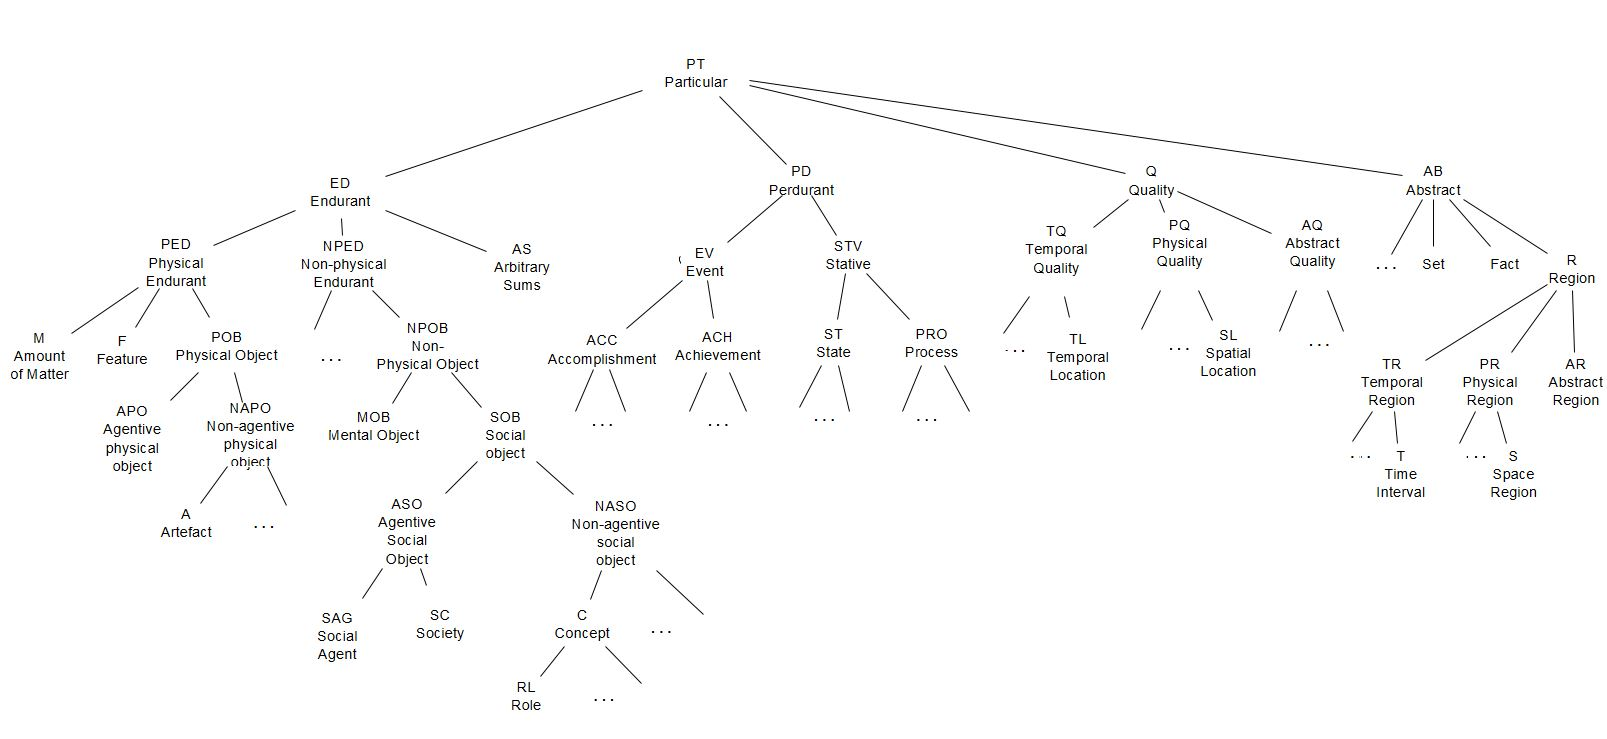
\includegraphics[width=\textwidth]{DOLCE-taxa-originalv2.JPG}
  \caption{\label{fig:DOLCE-taxa} \DOLCE taxonomy, taken from \cite{borgoDOLCEDescriptiveOntology2022}.   }
\end{figure}

\DOLCE qualities  were inspired by the trope theory~\cite{Campbell90} but differ from tropes in important ways. Qualities, for example the weight of a car and the color of a flower, are used for representing individual properties, i.e., specific properties of the individual objects in which they inhere. Thus, the weight property of a given car is specific to that car, which is called the {\em bearer} of that quality.
Each quality is itself an individual and `belongs' to its bearer. Consider a number of cars, say five. The colors of these five cars are five color qualities, one for each car, even though the five cars could be indistinguishable regarding their color.
Differently than tropes, qualities are associated to values and these can change in time. For example, the color quality of a flower can change its value as time passes: red in summer and brown in fall.
Indeed, values of qualities, called {\em quales}, are distinguished from qualities themselves. 
In this way, the assignment of values to qualities is flexible and follows the schema object-quality-quale (or bearer-individual quality-value).
In \DOLCE, qualities form the class $\generalStyle{Q}$ (whose predicate is written $\DOLCEQuality{\cdot}$) and the inherence relation is \quotes{quality-of} (written $\DOLCEQualityDirect{\cdot}{\cdot}$). A temporal quale relation associates a quality with some value which, as said, may be different at different times, and is written $\DOLCEQualeDirectTer{\cdot}{\cdot}{\cdot}$. 

We  introduce a further distinction, not present in \DOLCE, between \firstTimeKeyWord{intrinsic} and \firstTimeKeyWord{relational} (or extrinsic\footnote{
Note that the terms `relational' and `extrinsic' come from different research areas and are sometimes used with different meanings. 
}) qualities~\cite{sep-intrinsic-extrinsic}. 
Standard examples of intrinsic qualities are mass, length, and shape; of relational qualities are weight (which is relative to a gravitational field), the personal record for a marathon (which is relative to the social concept of marathon), and the distance of an object from another object (which requires the existence of both objects). 
Briefly, relational qualities are qualities of an object \textit{per se} that depend on other things like another object, the context or the environment.
To clarify our intuition we illustrate some of the previous examples: the distance of the Moon from the Earth, seen as a property of the Moon, cannot be thought of without considering the Earth, so we say that it is a relational quality of the Moon (similarly, for the distance of the Earth from the Moon). 
In contrast, if a certain brick has a given tensile strength, this fact does not depend on other entities, so that tensile strength is an example of intrinsic quality\footnote{Of course, one needs other entities to measure the tensile strength value, but note that this dependence is relative to establishing the value. The tensile strength exists independently of how one may measure it.}; similarly, other mechanical or chemical qualities, for example ductility or the structure of the atomic lattice in crystals, can be considered intrinsic. 
Another example is the difference between weight and mass of a body: the mass is intrinsic while the weight also depends on the position of the body in a gravitational field, e.g., if the body is on the Earth or on the Moon, which makes the latter quality relational. 
A more technical example is the voltage at a point of a component, which, since it is a potential, requires a second point used as  reference (the ground of the electrical circuit) in order to be meaningful. 
Informally speaking, capacities can be understood as having a relational nature, which explains our interest in the intrinsic/relational distinction across qualities. For, if we speak about the capacity of a device, say the capacity of a machine to process a certain number of items in a given time, then such capacity always refers to another entity, in this case the (prototypical) item.  Analogously, in \cite{qianFunctionBehaviorStructure1996}, Qian and Gero stated that there are different types of \quotes{behavioural variables}: structural, as the area of a room or the diameter of a water tap, and exogenous, as the water flow through a water tap. In the latter example, the water flow is an exogenous variable because \quotes{water is not part of the water tap design, it is only related to the design}, so that we could argue water is an additional entity required by the water flow quality of the tap, suggesting that this form of exogeneity can be captured via our notion of relational quality.  


In the previous examples, it seems that relational qualities are those qualities that depend, in some way, on an entity different (we say \firstTimeKeyWord{external}, see \refdf{def:external}) from their bearer. Unfortunately, the exact meaning of this dependence relation changes between the different examples. In particular, in the case of capacities the dependence is `potential', for a device can have the capacity to process a product, even when the product is not actually present. In contrast, in the case of relative distance the dependence is `actual', for a physical object is at any time at a certain distance from another.It follows that the characterisation of relational qualities is a complex matter that goes beyond the scope of this paper.\footnote{The interested reader can find a proposal on relational and intrinsic qualities in \cite{fonsecaRelationsOntologyDrivenConceptual2019}.} Therefore, we introduce intrinsic and relational qualities as primitive predicates that partition the class \DOLCE-qualities: 
\bflist
  \item[\myax{relationalQtPartialDef}] $ \RelationalQuality{x} \myfi \DOLCEQuality{x} $ 
  \item[\mydf{intrinsicQtPartialDef}] $ \IntrinsicQuality{x} \myiff  ( \DOLCEQuality{x} \land \neg  \RelationalQuality{x})$
  \eflist



Turning now to perdurants ($\DOLCEPerdurant{\cdot}$), in \DOLCE they are entities that are only partially present at any time they are present.\footnote{Ordinary physical objects such as cars, trees, rocks, etc. are fully present at every time in which they exist.} For example, a chemical process, the lifting of a load, and a sitting action are only partially present at each instant at which they happen. Indeed, the initial part of a chemical process is not present when the process reached the midway point, and vice versa.  \DOLCE uses three mereological properties to distinguish perdurants: cumulativity, homeomericity, and atomicity.
Cumulativity holds if the sum of two instances of a type has the same type, that is, if the type is closed under mereological sum. Consider, for example, \quotes{walking}: if we consider two walking activities, then the activity that comprises both is still an activity of type \quotes{walking}.
Cumulative perdurants\footnote{More precisely, instances of a cumulative type perdurant.} are called \firstTimeKeyWord{stative} ($\DOLCEStative{\cdot}$), while the ones that are never cumulative are called \firstTimeKeyWord{eventive}.
Homeomericity holds for a perdurant type if any parts of its instances are instances themselves.
This is the case of, e.g, \quotes{sitting}, since portions of a sitting action are still sitting actions.
Stative homeomeric perdurants are called \firstTimeKeyWord{states} ($\DOLCEState{\cdot}$), while the ones that are stative but have parts of different type are called \firstTimeKeyWord{processes}($\DOLCEProcess{\cdot}$). Walking itself is an example of process in \DOLCE: walking requires at least to complete a certain leg movement, below such granularity is not a walking movement.
Another example is the buzzing of a clapper (or buzzer): the clapper alternates between two states when clapping (opened/closed circuit), and neither state is per se of buzzing type. In \DOLCE the temporal relationship between a perdurant and the object participating in it is called \firstTimeKeyWord{participation}, written $\DOLCEPC{\cdot}{\cdot}{\cdot}$: in the previous example a participant of the buzzing is the clapper.


Coming to roles, they were not covered in \DOLCE originally. They have been introduced later as an extension \cite{masoloSocialRolesTheir2004}, and are now part of the expanded taxonomy \cite{borgoDOLCEDescriptiveOntology2022}.
Roles are antirigid and dependent (aka founded) classes \cite{guarinoOverviewOntoClean2009, guarinoFormalOntologyProperties2000,masoloSocialRolesTheir2004}. 
A class is antirigid whenever its instances are not necessarily so, and is dependent if all of its instances (existentially) depend on some external entity, often called context.
For example, a certain person can be a student, but no person is necessarily a student. Actually, we expect that a student ceases to be such after some time. 
In contrast, any person is necessarily a person, and is so independently of other external entities.
An ontological class (existentially) depends on, or is founded on, another if, whenever an instance of the first class is present, a corresponding instance of the second is present too.
For example, for every citizen there is a country, so that someone's citizenship depends on the country. Actually, in this paper, we will be more precise and distinguish between different kinds of dependence and founding, but the basic idea is still captured by the citizen-country example. 
Additionally, some authors divide roles depending on the type of their context, 
for example \cite{loebeAbstractVsSocial2007} distinguishes relational, processual, and social roles. The classification depends on whether the context is a relation, a process, or a social object. 
In \DOLCE, roles ($\DOLCERole{\cdot}$) are reified and considered as concepts ($\DOLCEConcept{\cdot}$), which themselves are a class subsumed by the class of non-agentive social objects ($\DOLCENASO{\cdot}$):
\bflist
  \item[\myax{roleSussum}] $ \DOLCERole{x} \myfi \DOLCEConcept{x}$
  \item[] \mytext{a role is a concept}
  \item[\myax{roleSussum2}] $\DOLCEConcept{x} \myfi \DOLCENASO{x}$
  \item[] \mytext{a concept is a non-agentive social object}
\eflist
In this paper, the fact that roles are founded is particularly important, thus, we give the following formalisation, where $\DOLCECLby{\cdot}{\cdot}{\cdot}$ (`classified-by', also called `play-as', if the first argument is a role) is the classification relation between a concept and its instances at a certain time, cf. \cite{masoloSocialRolesTheir2004}. In the formalisation we use some other relations taken from \DOLCE, namely: constitution, $\DOLCEK{\cdot}{\cdot}{\cdot}$,
 which is the  relation holding between some amount of matter and an object when the latter is made of the first (e.g., a statue and the amount of clay it is made of);  $\DOLCEOverTemp{\cdot}{\cdot}{\cdot}$, which is the usual temporal overlap relation (e.g., two semi-detached houses overlap because of the wall they share during the time they both exist); and $\DOLCEPRE{\cdot}{\cdot}$, which is the relation "being present (exist) at time". \bflist
\item[\mydf{external}] $ \external{x}{y} \myiff \neg (\DOLCEQualityDirect{x}{y} \lor \DOLCEQualityDirect{y}{x} \lor \exists t(\DOLCEK{x}{y}{t}) \lor \exists t(\DOLCEOverTemp{x}{y}{t}))$
\item[] \mytext{$x$ is external to $y$ if and only if $x$ is neither a quality of $y$, nor $y$ of $x$, nor $x$ is one of $y$'s constituents 
(at any time), nor $x$ and $y$ have parts in common\footnote{Substrata, parts, and qualities may not cover all possibilities especially if a different top-level ontology were used.} (at any time)}  
\item[\mydf{specificallyDependsOn}] $ \specificallyDependsOn{x}{y} \myiff (\exists t(\DOLCEPRE{x}{t}) \land \forall t(\DOLCEPRE{x}{t} \myfi \DOLCEPRE{y}{t}))$ 
\item[] \mytext{$x$ existentially depends on $y$ if and only if $x$ exists at some time and at any time when $x$ exists so does $y$}\footnote{The existential quantifier is a technicality: without it an entity that is never present would depend on all entities. Similarly, existential quantifiers are introduced in axioms having a similar structure to this one.}
\item[\mydf{foundingBasic}] $ \founded{x}{y} \myiff (\specificallyDependsOn{x}{y} \land \external{x}{y})$
\item[] \mytext{$x$ is founded on $y$ if and only if $x$ existentially depends on $y$ and $y$ is external to $x$} 
\eflist
Further, we specialize the founding relationship to concepts and their instances as follows:
\bflist
\item[\mydf{founding}] $ \foundedROLE{x}{y} \myiff (\DOLCEConcept{x} \land \DOLCEConcept{y} \land \exists z,t (\DOLCECLby{z}{x}{t}) \land \forall z,t (\DOLCECLby{z}{x}{t} \myfi \exists w (\external{z}{w} \land \DOLCECLby{w}{y}{t})))$
\item[] \mytext{the concept $x$ is instantiation-founded on the concept $y$ if and only if, whenever $z$ is a given entity that plays as $x$, 
there is also an external entity $w$ that is an instance of $y$} 

\item[\myax{roleFounding}] $ \DOLCERole{x} \myfi \exists y~ \foundedROLE{x}{y} $ 
\item[] \mytext{if $x$ is a role, then there is a $y$ on which it is instantiation-founded} 
\eflist 
For example, the role of `husband' ($x$) in \refdf{def:founding} is instantiation-founded on the concept of `marriage' ($y$), since every time a person ($z$) is a husband there is an individual marriage ($w$) between that person and another person,  which is external to the `husband' role: this means that there cannot be a husband if there is no marriage. 

We also need to capture a different kind of founding relation, that we call \firstTimeKeyWord{definition-founding} ($\foundedDef{\cdot}{\cdot}$). We do not formalize this relation as it requires discussing how to formally define roles, a topic beyond our concerns in this paper. We will use it with the following informal interpretation: \mytext{$x$ is definition-founded on some entity $y$ if and only if $y$ is used to define $x$}.
For example, if a doctor is defined as a person who treats sick people, then the doctor-role is definition-founded on the sick-person concept. 
Note that instantiation-founding and definition-founding need not  coincide. A person is a doctor even though, at a certain time, she is not treating any sick person: the doctor-role is not instantiation-founded on someone being in a sick state.

Finally, since roles, as well as concepts, can be seen as reified classes, there exists a specialisation relation between roles, which we write as $\DOLCEConceptSubsum{\cdot}{\cdot}$:
\bflist
\item[\mydf{conceptSussum}] $ \DOLCEConceptSubsum{x}{y} \myiff (\DOLCEConcept{x} \land \DOLCEConcept{y} \land \exists z,t (\DOLCECLby{z}{x}{t}) \land \forall z,t (\DOLCECLby{z}{x}{t} \myfi \DOLCECLby{z}{y}{t}) )$
\item \mytext{A concept $x$ specializes a concept $y$ if and only if all instances of $x$ are also instances of $y$} 
\eflist
For example, the role of the Italian Prime Minister specializes the role of Prime Minister.
{This notion of specialisation is admittedly weak. One would like to add a modal characterisation: definition \refdf{def:conceptSussum} should hold in all possible worlds. This problem applies to other definitions we introduce in this paper and is not ontological but related to the limitations of first-order logic. Without discussing logical technicalities, in this paper we will make use of these characterisations assuming that, in suitable systems, e.g. first-order modal logic, a suitable formula is substituted.}

\section{Modelling behaviours and functions in \DOLCE \label{sec:capabilitiesEtc}}
In this section we propose a framework to characterize how behaviour and function of engineering artifacts can be understood to make sense of the distinctions used by engineers in different areas, from engineering design to manufacturing and maintenance, from process planning and product planning to early system design planning. Within the following section, we will expand this view to capability and capacity.

In the literature, many terms are used to refer to engineering systems and devices such as part, component, tool, machine, (technical) artifact, functional object etc. 
We use \firstTimeKeyWord{technical artifact}\footnote{See \cite{borgoTechnicalArtifactsIntegrated2017} for a more in-depth discussion of technical artifacts.} to mean any physical object (see \refax{ax:subsumptionTArt}) that comes into being through an intentional technical process, such as, e.g., cars, planes, tooling machines and, more generally, devices designed to perform tasks. Also, we will use the terms \quotes{device} and \quotes{technical artifact} as synonyms. 
Additionally, we will use the term \firstTimeKeyWord{system} in order to highlight the mereological structure of a complex artifact. 
The notion of system is complex, cannot be reduced to  that of technical artifact, and its precise characterisation is an open problem (see e.g. \cite{mizoguchiRoleSystemicView2021}). In the paper, we take this notion as given introducing a primitive class, $\System{\cdot}$. In particular, technical artifacts belong to this class. 
The mereology mentioned above is built as usual from the temporalized parthood relation of \DOLCE,  $\DOLCEPart{\cdot}{\cdot}{\cdot}$. \DOLCE defines also a non-temporalized parthood relation, $\DOLCEPartBin{\cdot}{\cdot}$, given in \refdf{def:partConstant}. Axiom \refax{ax:part-present} and the class $\DOLCEPhysObj{\cdot}$, the category of physical objects, are also taken from \DOLCE.
\bflist
\item[\myax{subsumptionTArt}] $ \TechArt{x} \myfi \DOLCEPhysObj{x}$
\item \mytext{a tecnical artifact is a physical object}
\item[\mydf{partConstant}] $ \DOLCEPartBin{x}{y}  \myiff \exists t (\DOLCEPRE{y}{t}) \land \forall t (\DOLCEPRE{y}{t} \myfi \DOLCEPart{x}{y}{t})$
\item \mytext{$x$ is constantly part of $y$ if and only if whenever $x$ exists, it is part of $y$}
\item[\myax{part-present}] $ \DOLCEPart{x}{y}{t} \myfi (\DOLCEPRE{x}{t} \land \DOLCEPRE{y}{t})$
\item \mytext{if $x$ is part of $y$ at time $t$, then $x$ and $y$ are both present at time $t$}
\eflist




\subsection{Engineering behaviours}
Engineers create an artifact to realize a certain interaction between the artifact itself and elements of the environment. The behaviour of an artifact is the way in which that artifact participates in that interaction (e.g. \quotes{[the car] rattled when it hit the curve} ~\cite{chandrasekaranFunctionDeviceRepresentation2000}). 
In \DOLCE one models the happening of the interaction as a perdurant. How to ontologically understand behaviour is more tricky. 
In the literature, the term behaviour is used with different meanings, e.g., as simplified part or description of processes like in these excerpts: \quotes{The causal rules that describe the values of the variables under various conditions} \cite{chandrasekaranFunctionDeviceRepresentation2000}, \quotes{the behaviour represents objective conceptualisation of its input-output relation as a black-box} \cite{kitamuraOntologicalModelDevice2006}, \quotes{situation-independent conceptualisation of the change between input and output of the device} \cite{mizoguchiFunctionalOntologyArtifacts2009}. 
In \YAMATO \cite{Mizoguchi2017YAMATOYA} behaviours are modelled as processes with an \quotes{agent or an agent-like object as a doer}. 
Instead, in \cite{borgoFormalOntologicalPerspective2009} Borgo et al.  model them as relational qualities which characterize the specific way of participation of an object in individual events. 




  






Here we discuss a few key ontological properties to distinguish possible definitions of behaviour.
There are, in fact, at least four axes along which different meanings of behaviour can vary in the literature.
First, there is what we call the occurrence-property dichotomy:
\begin{itemize}
  \item behaviour can be something that happens in time  and in which the behaving entity participates, 
  in this case it is typically referred to as a transition between states or just as (staying in) a state. 
  Examples are provided by Goel \cite{goelStructureBehaviorFunction2009}, Chandrasekaran \cite{chandrasekaranFunctionDeviceRepresentation2000}, Umeda \cite{umedaFunctionBehaviourStructure1990}, and \YAMATO authors' \cite{mizoguchiFunctionalOntologyArtifacts2009}.
  \item behaviour can  be a quality, that is, something inhering into the behaving entity. 
   Examples are provided by Borgo et al.~\cite{borgoFormalOntologicalPerspective2009}, see also Vermaas or Gero and colleagues which talk of attributes or dispositions \cite{vermaasConceptualFrameworkJohn2007,geroCategorisingTechnologicalKnowledge2002}.
\end{itemize} 

Then, there is the token-type distinction: behaviour can be a class or a concept, as for  Mizoguchi in \cite{mizoguchiFunctionalOntologyArtifacts2009}. Alternatively, it can be an instance of something, or an entity relative to a specific event, as for Chandrasekaran and Josephson in \cite{chandrasekaranFunctionDeviceRepresentation2000}, and for Borgo et al. in \cite{borgoFormalOntologicalPerspective2009}, respectively. 

Additionally, there is the external-internal axis, that is, the behaviour of an artifact may refer only to characteristics of the artifact itself, or it may need to refer to  external entities.
For example, `the electric switch can alternate between open and closed states' is an internal behavioural description, as it refers only to transitions between states of the artifact.
In contrast, `the current passing through an open switch is zero, if the applied voltage stays within operating conditions' is an external description, since, the current and the voltage are not intrinsic elements of the artifact. Some authors explicitly use behaviour with the internal meaning, e.g. Zhao et al. in \cite{zhaoStateBehaviorFunction2019}, others with the external one, as Kitamura et al. in \cite{kitamuraOntologybasedSystematizationFunctional2004}.

Finally, there is the modal axis, since behaviours can be either expected (i.e. as envisioned by engineers) or actual (i.e. what actually happens), as implied by Gero in \cite{geroSituatedFunctionBehaviour2004} with respect to design activity (though one could use the same duality when talking of, e.g., malfunctioning).
This axis includes, arguably, talks of causal laws or relations, since those could be conceptualized as changes of a system under some kind of 
modality, that is, changes that necessarily happen when some condition is met.
We do not argue in favor of conceptualizing causal laws in this way, but, in any case, one must also take this use of behaviour into account, since it is encountered often. 




















\medskip
In this paper, we take an \firstTimeKeyWord{engineering behaviour} to be a \DOLCE perdurant with a few assigned roles. 
The class of engineering behaviours, called just behaviours from now on, is the class of perdurants in which one can identify two `processual'\footnote{Note that the term \quotes{processual role} refers to general perdurants, it is not limited to \DOLCE processes. The terminology is taken from Loebe which introduces it relatively to the GFO approach \cite{loebeAbstractVsSocial2007}.} roles in the sense of \cite{loebeAbstractVsSocial2007}: an active one, called \firstTimeKeyWord{doer}, and a passive one, called \firstTimeKeyWord{operand} or \firstTimeKeyWord{flow} \cite{pahl_engineering_2007}.
This role-based notion of behaviour is motivated by (and restricted to) the domain of functional modeling where it highlights a common engineering viewpoint. This notion complements the broader ontological view of behaviour as a relational quality between an entity and its environment, which was introduced in~\cite{borgoFormalOntologicalPerspective2009}.
While the role-based view introduces behaviour as a perdurant and fits naturally with the view of ontological function that we will investigate later, the ontological notion of behaviour can be resumed to distinguish the behaviour of the doer from that of the operand, if necessary.
For instance, a cutting action entails that there is something that is the subject of the action, say a saw (or the system formed by a person or machine using the saw), and the object of the action, say a beam of wood. At the same time, the saw has its own specific way to interact with that environment (to which the wood belongs), i.e., its own ontological behaviour, and so does the wood with respect to its environment (to which the saw belongs).
The same holds for pumping, joining, and other behaviours described by transitive verbs. 

All devices' engineering behaviours that can be described as operations on operands have engineering behaviours as described above. 
Such behaviours, whose class we characterize with predicate $\BehaviourConcrete{\cdot}$, are external behaviours, since the flow is an entity external to the behaving artifact (the doer).
We conceptualize the two processual roles through two specialisations of the participation relation: $\participateAsDoer{\cdot}{\cdot}{\cdot}$, to indicate participation in a process with the role of an agent or agent-like doer, and $\participateAsFlow{\cdot}{\cdot}{\cdot}$, for the role of flow: 
\bflist
  \item[\myax{participateAsDoerRage}]  $ \participateAsDoer{x}{y}{t} \myfi (\TechArt{x} \lor \DOLCEAgent{x} ) \land \BehaviourConcrete{y} \land \DOLCEPC{x}{y}{t}$
\item \mytext{if $x$ is a doer in $y$ at time $t$ then $x$ is a technical artifact or an agent, $y$ is a behaviour, and $x$ participates in $y$ (in the \DOLCE sense) during that time}
  \item[\myax{participateAsFlowRage}]  $ \participateAsFlow{x}{y}{t} \myfi \BehaviourConcrete{y} \land \DOLCEPC{x}{y}{t}$
\item \mytext{if $x$ is a flow in $y$ at time $t$ then $y$ is a behaviour, and $x$ participates in $y$ during that time}
\item[\myax{processualRoles}] $ \BehaviourConcrete{x} \myfi \exists y,z,t(\participateAsDoer{y}{x}{t} \land \participateAsFlow{z}{x}{t} \land y \neq z) $ 
\item \mytext{$x$ is a behaviour only if there are at least a doer and a flow that participate in $x$}
\eflist

From \refax{ax:processualRoles} it follows that behaviours are perdurants. Additionally, we assume that behaviours can be combined to give causal explanations of complex perdurants (e.g. the beam was cut, therefore it fell to the floor), and formalize this with a binary relation called \firstTimeKeyWord{causal contribution}\footnote{This relation among perdurants is inspired by the one introduced in \YAMATO \cite{mizoguchiYAMATOAnotherMore}. Note that the latter is limited to \YAMATO processes.}, which we assume holds more in general between perdurants:
\bflist
  \item[\myax{contribRange}] $ \causallyContr{x}{y} \myfi \DOLCEPerdurant{x} \land \DOLCEPerdurant{y} $
\eflist

We do not axiomatize the causal contribution relation further as it has a much broader scope than the focus of this paper but see~\cite{borgoFirstorderFormalizationEvent2014} for an initial proposal.\footnote{Note that Borgo and Mizoguchi constrain the relation of causal contribution so that its domain and range are processes. In \cite{mizoguchiUnifyingDefinitionArtifact2016}, the authors argue that the same relation can also apply to a process and a state, with the convention that, whenever that happens, it holds between the first process and the process of achieving the state.
Here, we take a broader view and set the domain and range to be the category of perdurants.}
Similarly, we do not axiomatize the roles of doer and flow, see~\cite{loebeAbstractVsSocial2007} for a deeper discussion of these notions.

The role-based approach combined with the causal contribution relation allows us to model behaviour from the point of view of the participating device 
\refax{ax:processualRoles}. Admittedly, it also introduces some limitations. For instance, the case of an artificial agent changing its own setting exemplifies a function where doer and flow coincide, a case ruled out by \refax{ax:processualRoles} (such a function is called `change over' in \cite{borgoKnowledgebasedAdaptiveAgents2019}).
A full analysis of the relationships between the two approaches to behaviour (relational quality vs. perdurants with roles) has not been carried out. We highlight once more that they are mutually compatible within \DOLCE. When using behaviour from now on, we will mean engineering behaviour unless otherwise specified.


Having conceptualized behaviours as a role-based view of perdurants, we spend a few words about the notion of state of an engineering system.
In \DOLCE states are, as mentioned in Section \ref{sec:DOLCE}, cumulative and homeomeric perdurants.
The same properties should hold for engineering system states.
Indeed, if we understand states, as many engineers do, as conditions determined by constraints over state variables, then such conditions are homeomeric (if a device satisfies a constraint over a time period, then it also satisfies it during a fragment of that period) and cumulative (if a device satisfies a constraint over some time periods, then it satisfies it during the union of those periods).
Unfortunately, engineers commonly use the term \quotes{state} also for oscillating phenomena and the like (e.g. the buzzing action of a clapper, which alternates between two different \DOLCE-states while buzzing, namely open-circuit and closed-circuit). 
Hence, the right \DOLCE category to conceptualize system states is the one of stative perdurants. 
To avoid a terminological clash, in the following we will use the term \quotes{state} following the engineering terminology. Ontologically, it is to be understood as a \quotes{stative condition} in \DOLCE. For this reason, we will use the stative predicate $\DOLCEStative{\cdot}$ in formulas.

Finally, engineers typically know how to characterize a state a system should be in, therefore we assume that, given a technical artifact, some `types' of states are selected as desired, and call them \firstTimeKeyWord{goals}. Note that, typically, one selects the conditions that a state has to satisfy, that is, selects a concept 
and not a state-instance, since the latter would have a specific time extension. 
Hence, we have that
\bflist
\item[\myax{goalSubsum}] $ \Goal{x} \myfi \DOLCEConcept{x} \land \forall y,t (\DOLCECLby{y}{x}{t} \to \DOLCEStative{y})$
  \item \mytext{a goal is a concept that classifies stative perdurants only}
\eflist
Thus, goals may correspond to expressions \quotes{the temperature at the port B of the heat exchanger is between 80 and 110 Celsius degrees} and \quotes{the buzzer is clapping with a frequency of at least 10kHz}, which are expressions for state classifiers.



\subsection[Two types of functions]{Systemic functions and \ontoFunc{fullPlural}} 
\paragraph{Systemic functions.}
In this paragraph we exploit the concepts introduced in the previous sections and propose a preliminary formalisation of \ontoFunc{fullPlural} as roles. 
Precisely, we start by defining \firstTimeKeyWord{systemic functions}. In doing that, we are mainly inspired by the definition presented in \cite{mizoguchiUnifyingDefinitionArtifact2016} (cfr. also Cummings' definition in \cite{cumminsFunctionalAnalysis1975}), from which we also take the concept name.
Such a definition is based on the so-called \firstTimeKeyWord{systemic view} of devices, that is, on the idea that devices are complex aggregates of components, whose interaction with the rest of the system contribute to generate the activity of the whole system. 
In this context, a function is seen as the contribution of an individual component's activity to the activity of the system as a whole, and teleological aspects are introduced through goals imposed on the system. Note that our notion of  behaviour (a perdurant with roles) is different than the one in~\cite{mizoguchiUnifyingDefinitionArtifact2016} and presents a nice feature: with our approach it is very simple to decompose (and to recompose) the system's behaviour into components' behaviours as the latter are simply parts of the first (provided one correctly identifies the suitable roles).

\bflist
  \item[\mydf{functionOf}] $ \FunctionSysOf{x}{y} \myiff (\DOLCERole{x} \land 
  \exists z,g,b,t (\System{z} \land \goalOf{g}{z}  \land  \DOLCECLby{b}{x}{t} \land \DOLCEPart{y}{z}{t} \\ \land
    \forall b',t' (\DOLCECLby{b'}{x}{t'} \myfi (\BehaviourConcrete{b'} \land 
      \participateAsDoer{y}{b'}{t'} \land \DOLCEPart{y}{z}{t'} \\ \hfill{} \land \causallyContr{b'}{g}))))  $ 
  \item \mytext{$x$ is a systemic function of $y$ if and only if $x$ is a role and there exist a system $z$ and a goal $g$ for $z$ such that $x$ classifies only behaviours which have $y$ as doer and part of $z$, and that causally contribute to achieve $g$}\footnote{This means that the term \quotes{systemic} in \quotes{systemic function} refers to the dependence of such role-concept to a system, and does not imply that the player artifact is a system itself. For example, if a wood table is held together by screws, each screw has a systemic function in the table-system: it connects one of the table-legs to (a side of) the table-top, even though none of the screws is a system.}
  
  \item[\mydf{function}] $ \FunctionSys{x} \myiff \exists y ~\FunctionSysOf{x}{y}$
  \item \mytext{$x$ is a systemic function if and only if it is the systemic function of some object $y$}
\eflist

Of course, there are many different function conceptualisations in the literature and each is relevant from one engineering perspective or another. We propose to start from Definition \refdf{def:functionOf} because, differently from the others, it is ontologically clear and helps to clarify the assumptions on which other meanings rely.

Note that, observing Definitions \refdf{def:functionOf} and  \refdf{def:function}, it is natural to assume that systemic functions are definition-founded on systems, a fact that we introduce with the following axiom:
\bflist
\item[\myax{functionSys-founded}] $ \FunctionSys{x} \myfi \exists y (\System{y} \land \foundedDef{x}{y}) $  
\item \mytext{each systemic function is definition-founded on some system}
\eflist

\paragraph[meta]{\ontoFunc{fullPluralCapital}.}
In engineering practice, one may speak about functions independently of any system, for instance in an early system design phase. 
For example, if one wants to address the problem of finding the set of devices that have the capability
of realizing a needed transformation, the devices cannot be \textit{a priori} associated with a certain system, since there is no system yet. Indeed, the system is a variable input of the problem.
Therefore, to solve this problem, a more general concept of function is needed, see, e.g., \cite{borgoKnowledgebasedAdaptiveAgents2019}. 
We call such functions \firstTimeKeyWord{\ontoFunc{fullPlural}} as they are relative only to the upper ontology one is using. The idea is that these functions distinguish very general transformations without addressing how such a transformations may occur or to which entities they apply. The informal intuition of \ontoFunc{fullPlural} is that they are classified primarily according to the ontological difference(s) they enforce between the input and the output states. In this sense, they are independent of systemic functions. 

For instance, assume we want to model a walking activity as the realization of a moving function. Walking may be considered a simple action but is very complex to model since it is a highly coordinated, continuous and dynamic process. One might decide to simplify its modeling by \qquotes{restricting} the walking model to some aspects, such as the variation of the distance of the feet from the floor, the trajectory of the body's center of mass, the changing contact forces between the feet and the floor, those developing into the leg joints, and so on (cf. \cite{guarinoEventsTheirNames2022}). 
It turns out that there are many aspects that one may focus on. 
Which should one use? 

Assuming that an upper ontology is fixed (\DOLCE in this paper), one considers the state transitions that are made available by the ontology and that are relevant to the transition of interest. 
In the case of walking, the relevant feature(s) that characterize a walking in the upper level of \DOLCE are the change of location of the entity. At this high level, among the entities relevant to walking, the ontology makes available only space and location qualities. Other classes, like foot or center of mass, and other qualities, like speed and force, are not characterized nor committed to. The perdurant could not be said to be a walking since \DOLCE has no walking category nor the needed ontological commitments to introduce such a category. If walking at this level can be characterized only by the change of the location quality, then one cannot distinguish it from swimming or flying (this depends on the upper level ontology, different ontologies may be more or less rich). One may wonder whether this level of characterization is too weak to be used for functional modeling. It is not. Already at this level one can make substantial differences since one can distinguish cutting from walking. Cutting is characterized by the presence of one entity at the initial state and two or more at the final state, walking is not. (In \DOLCE, like most (perhaps all) upper ontologies, entities can be distinguished in number, thus cutting and walking are different types of perdurant even at this level.) 
Since functions are realized by perdurants, we can use this ontology-driven categorisation of perdurants to introduce a categorisation of functions.
Let us call \ontoFunc{fullPlural} the functions that are carried out by transformations characterized by the ontological commitments (thus, distinctions) present in the upper ontology. As said, this provides only a high level (coarse) characterization of functions.
Since the resulting taxonomy of functions strictly depends on the ontology adopted, we use the qualifier \qquotes{ontological} 
and call them \ontoFunc{fullPlural} (where more than one upper level ontology is used, one should be more precise indexing the \ontoFunc{fullPlural} by the ontology they depend upon, e.g., `\DOLCE-ontological functions'). 
Continuing the discussion with \DOLCE as the upper ontology, the ontology makes available the categories \textit{region}, \textit{quality}, \textit{physical object}, \textit{amount of matter}, etc. (see Figure \ref{fig:DOLCE-taxa}), which give rise to several \ontoFunc{fullSingular}-types based on \textit{change in quality-value} (for example, \textit{the controller increased the internal temperature of the oven}), \textit{change of physical object} (e.g., \textit{the employee assembled four legs and a table-top to form a table}), \textit{change of amount of matter} (e.g., \textit{the water was vaporized by the boiler}), and so on, see Figure \ref{fig:onto-func-taxa}.

\begin{figure}
  \centering
  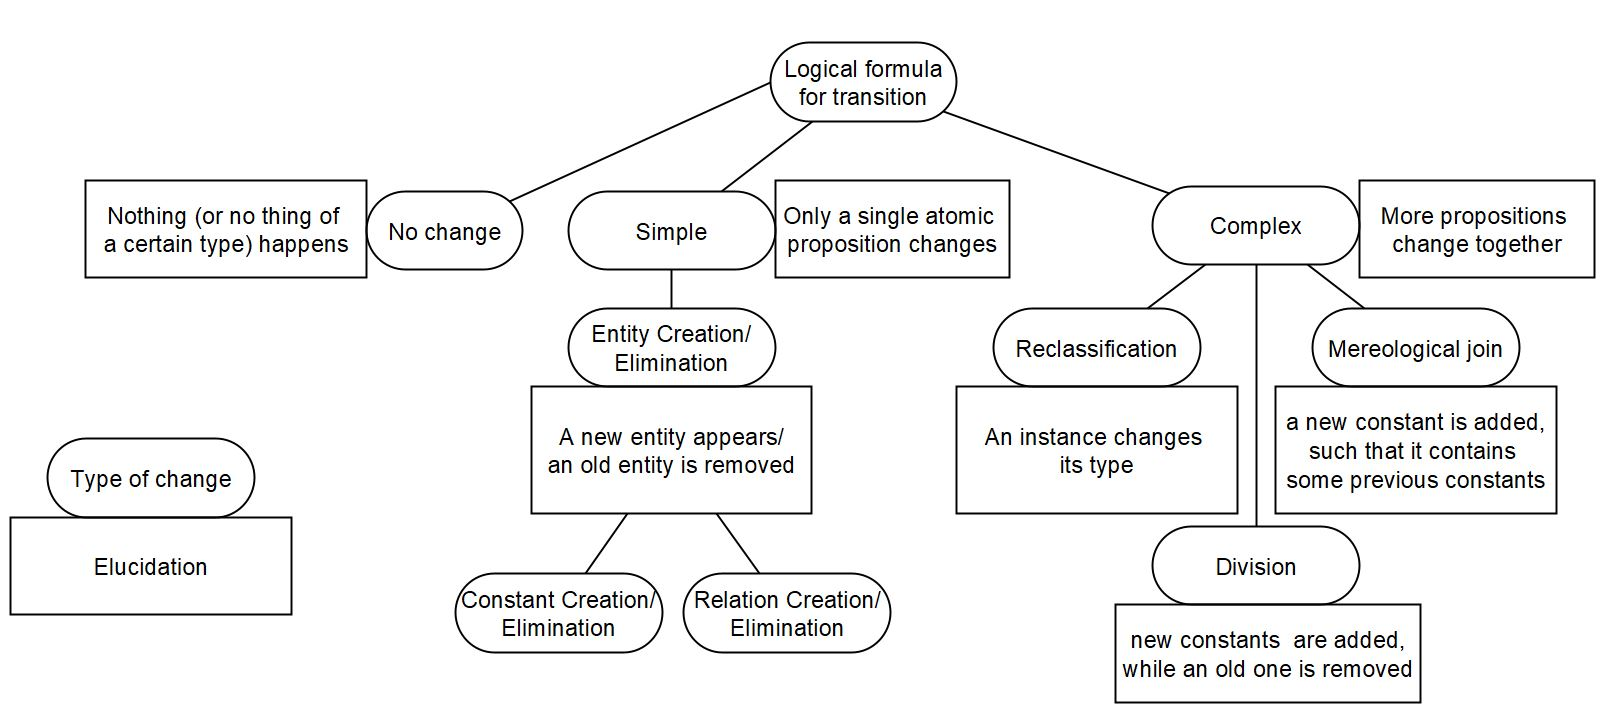
\includegraphics[width=\textwidth]{onto-func-logic-nocolor.JPG}
  \caption{\label{fig:onto-func-logic} A non exhaustive taxonomy of the logical formulas describing changes between states, classified depending on what predicates differ between the initial and final states.}
\end{figure}
\begin{figure}
  \centering
  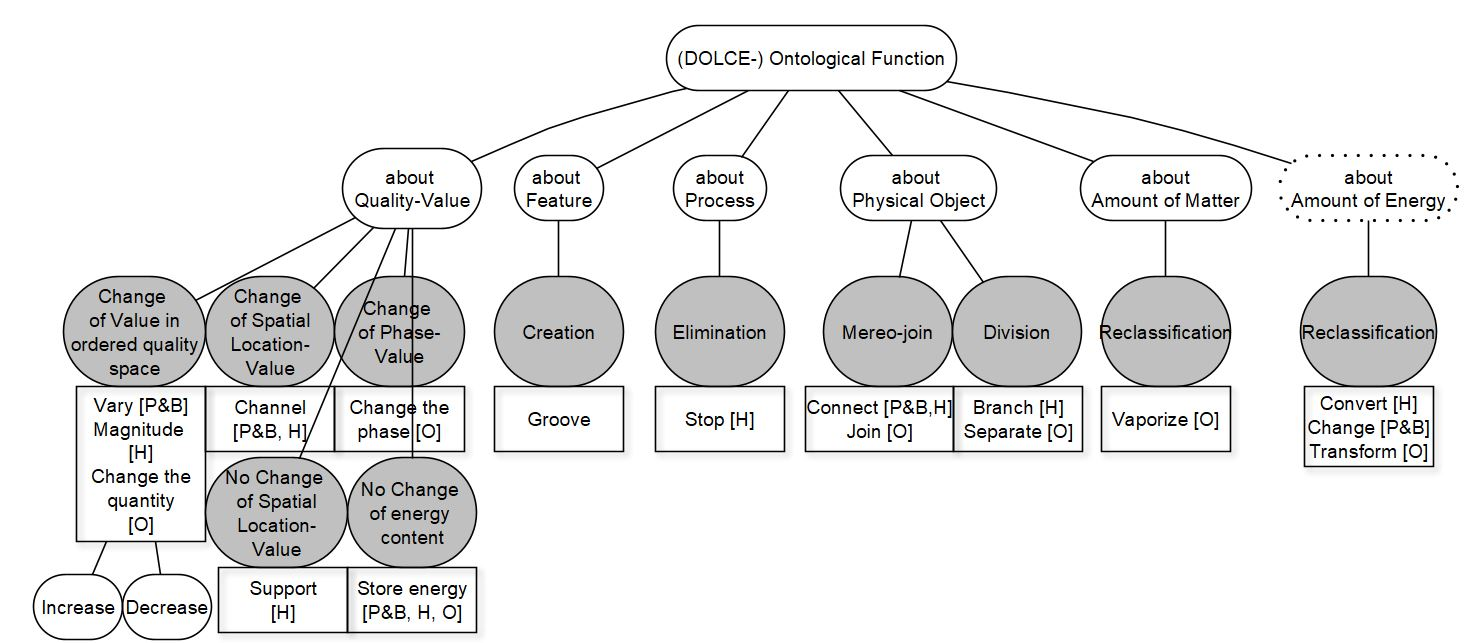
\includegraphics[width=\textwidth]{onto-func-taxav2-nocolor-v2.JPG}
  \caption{\label{fig:onto-func-taxa} An example of how a taxonomy of \ontoFunc{fullPlural} could be organized. The rounded white rectangles contain the \ontoFunc{fullPlural}-categories (classes of perdurants with identified doer and flow roles). The gray circles are functional concepts used to specialize \ontoFunc{fullPlural} as in \refdf{def:ontoDef1}, and refer to Figure \ref{fig:onto-func-logic}. The rectangles with sharp corners list alternative terms used in the literature to label that functional concept: H, P\&B, and O refers to \cite{hirtz_functional_2002}, \cite{pahl_engineering_2007}, and \cite{sasajimaFBRLFunctionBehavior1995}, respectively. (Notice that terms may occur in the literature also with different meanings than in this figure.) 
  The same perdurant may be classified by more than one functional concept.
  `Amount of Energy' is listed only for the sake of example, it is not part of DOLCE.}
\end{figure}

Note that an ontological category can be involved in a transition in different ways. 
For example, an instance of said category could be eliminated, meaning that the instance was present in the state before the transition but not after, or an instance could be created, meaning that the instance was not present before a transition but exists after.
Another possibility is that there is a change of a relation of the ontology, e.g., in the initial state there were two individuals that were, say, one part of the other, while in the final state they are not.
More complex changes can be described, depending on the difference between the initial and final structure of the ontology. Note also that in most cases the same event may be classified by several \ontoFunc{fullPlural}. For instance, an event of cutting by a device, say a knife, is also a squeezing event, i.e., a compression (a change of the shape quality of the initial object) and a moving event (a change of the device location relatively to the object's location). Clearly, most of these distinctions are similar to those obtained via the ontological analysis of events~\cite{guarinoEventsTheirNames2022}.
We have reported some of these cases in Figure \ref{fig:onto-func-logic}, which is not exhaustive.
Finally, the functional terminology used in this paragraph is  inspired by engineering literature which, as we have seen earlier, is not homogeneous. 
For instance, the \firstTimeKeyWord{reclassification} (i.e., a change such that an instance changes type) of energy or matter is in other places called \quotes{convert} \cite{hirtz_functional_2002, sasajimaFBRLFunctionBehavior1995} or \quotes{change} \cite{pahl_engineering_2007} or \quotes{transform} \cite{kitamuraOntologybasedSystematizationFunctional2004}, while the change of value of a spatial location quality is called \quotes{channel} \cite{pahl_engineering_2007,hirtz_functional_2002}, and so on.


Functional terms that are linked to domain-level terms (e.g., \quotes{vaporize}, \quotes{moisten}, \quotes{heat})
are not captured at the lever of \ontoFunc{fullPlural} and require a domain or middle-level ontology containing corresponding concepts (e.g., vapour, humidity, temperature) in order to expand the construction we have just described up to that level of ontological distinctions. 
The ontological nature of some concepts, like \quotes{energy}, 
is unclear \cite{mcginnOntologyEnergy2012} despite being a fundamental concept in engineering and physics. 
Nonetheless, given an ontology containing a conceptualisation of energy, it is possible to introduce a corresponding \ontoFunc{fullSingular}, which might be different in another ontology with a different conceptualisation of energy.
For instance, one could conceptualize energy as a quality, as done in~ \cite{borgoFormalizationFunctionsOperations2011}. 
This is the case, arguably, when one speaks about the energy \textit{of something}, e.g, of a battery.
In this case, in our ontology there would be a, say, \textit{energy content} quality-type, which gives rise to a corresponding \textit{convert energy} ontological function.
Another possibility is to conceptualize energy as an endurant, which can reside into entities, change its location, and change type (e.g., heat energy, kinetic energy, etc.).
In that case, the \textit{convert energy} ontological function would be a reclassification-type transformation.

Formalizing \ontoFunc{fullPlural}, like formalizing events, might be difficult. One would benefit from the introduction in the ontology of a general relation `change of \ldots in event \ldots'.
An ontological function, as understood in this paper, is essentially an event classifier which looks at what changes (or remains stable) in the event. 
This suggests defining specific functions by comparing, for instance, initial and final states. For example, a \textit{connect} function could be introduced as follows:
\bflist
  \item[\mydf{connect}] $ \Connect{x} \myiff (\DOLCECLbyBinary{y}{x} \myiff \DOLCEEvent{y} \land \exists a,b,c,s_i,s_f,t_i,t_f~(\sState{y}{s_i}{t_i} \land \eState{y}{s_f}{t_f} \land \Goal{s_f} \land \DOLCEPhysObj{a} \land \DOLCEPhysObj{b} \land \DOLCEPhysObj{c} \land \DOLCEPC{a}{s_i}{t_i} \land \DOLCEPC{a}{s_f}{t_f} \land \DOLCEPC{b}{s_i}{t_i} \land \DOLCEPC{b}{s_f}{t_f} \land 
  \DOLCEPC{c}{s_f}{t_f} \land \DOLCEPart{a}{c}{t_f} \land \DOLCEPart{b}{c}{t_f}) \land \neg \exists c' (\DOLCEPhysObj{c'} \land \DOLCEPC{c'}{s_i}{t_i} \land \DOLCEPart{a}{c'}{t_i} \land \DOLCEPart{b}{c'}{t_i})) $ 
    \item[] \mytext{A \textit{connect} function is a classifier of events that are transitions between a starting state ($s_i$, with time extension $t_i$) and a final state ($s_f$, with extension $t_f$) and two entities ($a$ and $b$) participate in such states such that in the final state, but not in the starting one, they form a single object ($c$)}
\eflist 
In the previous formula we used the predicate $\sState{y}{s_i}{t_i}$ to mean that $s_i$ is a state with time extension $t_i$, which is part of the perdurant $y$ and such that there are no parts of the time extension of $y$ which precede $t_i$. Analogous meaning for $\eState{\cdot}{\cdot}{\cdot}$.
Notice that: $(a)$ this notion captures the act of forming a single object out of two given ones, to formalize an assembly function one should add the condition that the final object is also a single piece (self-connected); $(b)$ if one reverses the initial and final states in Formula \refdf{def:connect}, then one obtains a definition for the \textit{divide} function.


Another example, to define a \textit{convert} function (here $\Phi$ and $\Psi$ are types belonging to the set $\mathcal{NR}$ of all non-rigid types of the underlying ontology): 
\bflist
  \item[\mydf{convert}] $ \Convert{x} \myiff (\DOLCECLbyBinary{y}{x} \myiff \DOLCEEvent{y} \land \exists s_i,s_f,t_i,t_f,a,\Phi,\Psi~(\sState{y}{s_i}{t_i} \land \eState{y}{s_f}{t_f} \land \Goal{s_f} \land \Phi\in\mathcal{NR} \land \Psi\in\mathcal{NR} \land \Psi\cap\Phi = \emptyset \land  \DOLCEPC{a}{s_i}{t_i} \land \DOLCEPC{a}{s_f}{t_f} \land \Phi(a,t_i) \land \Psi(a,t_f))) $ 
  \item[] \mytext{A \textit{convert} function is a classifier of events that are transitions between a starting state ($s_i$, with time extension $t_i$) and a desired final state ($s_f$, with extension $t_f$) and, moreover, there is an entity ($a$) that at time $t_i$ is instance of a type ($\Phi$), while at time $t_f$ is instance of a different, disjoint, type ($\Psi$).}
\eflist 
Notice that in the previous definition we have quantified over the set of all non-rigid classes of an ontology ($\mathcal{NR}$). 
If such a set is finite, like in \DOLCE, then the quantification corresponds to a finite disjunction of predicates, therefore Formula \refdf{def:convert} is a first-order formula.
Moreover, upper-level ontologies typically contain only rigid categories (e.g., if an individual is a physical object, it is always a physical object), therefore, such a convert function becomes useful when modelling changes in entities that go through phases \cite{guarinoOverviewOntoClean2009}, when modelling entities that change their processual role (as described earlier) or in combination with non-rigid categories (as provided by middle or domain-level ontologies).

The type of all \ontoFunc{fullPlural} that involve some change in quality values (cf. qualitative events in~\cite{guarinoEventsTheirNames2022}) could be defined as follows:
\bflist
  \item[\mydf{changeQualityValue}] $ \ChangeQualityValue{x} \myiff (\DOLCECLbyBinary{y}{x} \myiff \DOLCEEvent{y} \land \exists s_i,s_f,t_i,t_f,a,q,v_i,v_f~(\sState{y}{s_i}{t_i} \land \Goal{s_f} \land \eState{y}{s_f}{t_f} \land \DOLCEQualityDirect{q}{a}{t_i} \land \DOLCEQualityDirect{q}{a}{t_f} \land v_i \neq v_f \land \DOLCEPC{a}{s_i}{t_i} \land \DOLCEPC{a}{s_f}{t_f} \land \DOLCEQualeTer{q}{v_i}{t_i} \land \DOLCEQualeTer{q}{v_f}{t_f})) $ 
  \item[] \mytext{A \textit{change of quality-value} function is a classifier of events that are transitions between a starting state ($s_i$, with time extension $t_i$) and a desired final state ($s_f$, with extension $t_f$) with a participating entity ($a$) which has a quality ($q$) with different values, $v_i$ and $v_f$, at times  $t_i$ and $t_f$, respectively.}
\eflist
One can further specialize this latter notion. If the quality in formula \refdf{def:changeQualityValue} is spatial location, the \ontoFunc{fullSingular} will be of type \textit{channel}.
If the quality in \refdf{def:changeQualityValue} takes values in an ordered space (e.g., \textit{temperature}, \textit{humidity}, etc.) then the \ontoFunc{fullSingular} is of type \textit{vary}, possibly specialized into \textit{increase} and \textit{decrease} types, see \cite{hirtz_functional_2002,pahl_engineering_2007}. 
Some functions, such as \textit{store} and \textit{support}, hint at the absence of change: for instance, a battery stores energy very well if it does not lose its charge over time, while a load-bearing wall supports the roof only if the roof does not fall. 
Therefore, functional concepts like store and support could be defined by modifying formula \refdf{def:changeQualityValue} to impose that the initial and final values of the quality are the same (perhaps including some tolerance).

At this point we make three observations: 
\begin{itemize}
  \item By construction, ontological functions cannot be fine grained. On the one hand, they are limited to the language of the upper ontology. On the other hand, they do not consider at what happens between the initial and final states. Take, for example, a temperature-controlled oven. 
  The controller unit of the oven makes it so that the temperature in the oven stays, up to some tolerance, at a target value.
  The controller could achieve this by switching off the heat when the temperature is above the target value, and by switching on when the temperature is below the target. 
  The temperature value oscillates around the target value, and such a process cannot be deduced by only observing the differences between the initial and final states.
  Therefore, events that maintain a stable temperature vs. events in which it oscillates cannot be distinguished by \ontoFunc{fullSingular} unless one enriches the function definitions by allowing further conditions to constrain the temperature value during the event (e.g., via variation patterns, see \cite{guarinoEventsTheirNames2022}).
  This is in line with our view of \ontoFunc{fullPlural} but recall that one should consider only conditions that are expressible within the language of the ontology. 
  \item Events can be very complex and participated by many relevant entities (e.g., walking from a biomechanical point of view). 
  This, together with the fact that we admit also \ontoFunc{fullPlural} defined by the absence of some type of change (e.g., \textit{support}), makes so that many events would be classified by a combination of \ontoFunc{fullPlural} (as observed earlier while discussing the cutting example).
  This is not unexpected, and, in fact, reflects the flexibility of teleological thinking.
  Take, for example, a load-bearing wall.
  One could say that its function is to \textit{support} the weight of the roof, but it may also \textit{transmit} the load to the floor, or even \textit{stop} the wind from entering the house, or \textit{divide} the space inside the house into smaller rooms, and so on. 
  To recognize what aspect is the most relevant in a given context is a task for the engineer or technician, which, using a contextual viewpoint, determine what aspects to focus on and thus the target function. This is the reason for using the term `function' (in combination with `ontological') to characterize these classifiers.
  Events, by their nature, are open to different interpretations. 
  \item Lastly, we argue in favour of the flexibility of \ontoFunc{fullPlural}.
  In the previous paragraphs, we have mainly used functional terms taken from the Functional Basis \cite{hirtz_functional_2002} or from the influential view of \cite{pahl_engineering_2007}.
  Such vocabularies are indeed capable of expressing a vast quantity, if not the totality, of functions used within engineering domains, but they may not do so in the most natural way.
  For example, suppose that one is working with tooling machines that cut holes, slots, grooves, etc. in the workpieces. 
  Then, using the Functional Basis one is reduced to using just the term \textit{remove} to talk about the functions realizing such features in the workpiece.
  Instead, if one uses a domain ontology that contains concepts such as hole, slot, groove, etc., then one can build corresponding functional terms, say \textit{make hole}, \textit{make slot}, \textit{to groove}, etc., defined analogously to the previous formulas.
  Such terms may be more natural than just using \quotes{removing}, and may even differ significantly  from \quotes{removing}, depending on their precise formalisation.
  Another example: in the Functional Basis vocabulary, the term \quotes{stop} means \quotes{to cease the transfer of a flow}, for instance \quotes{A reflective coating on a window stops the transmission of UV radiation through a window} \cite{hirtz_functional_2002}. But what if perdurants are important in our domain and we want to say that something \textit{stops a process} (e.g., \qquotes{The addition of a respiratory inhibitor stops the absorption of amino acids}, not that \qquotes{stops the amino acid-material-flow from moving}, but that it \qquotes{stops the absorption}, where absorption is an important element of the domain?
  We could derive useful functional terms, from an appropriate domain ontology managing concepts of domain processes.
\end{itemize}

Up to this point we have defined some types of \ontoFunc{fullPlural}, but not the concept of \ontoFunc{fullSingular} itself. 
A possibility is to find an exhaustive list of types of \ontoFunc{fullPlural} and then define \ontoFunc{fullSingular} as the disjunction of all those types, for instance:
\bflist
  \item[\mydf{ontoDef1}] $ \FunctionAbs{x} \myiff (\Connect{x} \lor \Divide{x} \lor \Convert{x} \lor \dots) $
\eflist
This can be done by providing an exhaustive list of ontological functions made available by an upper ontology.
Another possibility is to look for an intrinsic definition of \ontoFunc{fullPlural} that informally could be as follows:
\bflist
  \item[\mydf{ontoDef2}] \mytext{A concept is a \ontoFunc{fullSingular} if and only if it classifies exactly those events consisting in a transition such that the changes (or the absence thereof) between the initial and final states (or across the whole transition) is characterized in terms of a formula expressed in the language of an upper ontology.}
\eflist
Since \qquotes{a formula expressed in the language of an upper ontology} is not something that can be written in a natural way using first-order logic, we cannot give an intrinsic first-logical definition of \ontoFunc{fullPlural}. (A similar argument could be applied to extend the notion of ontological functions to functions in the language of reference ontologies.)


\paragraph[meta]{Link between systemic functions and \ontoFunc{fullPlural}.}
Returning to the relation between systemic functions and \ontoFunc{fullPlural}, we observe that the former correspond to system-dependent functional descriptions, while the latter corresponds to system-independent functional descriptions. 
Since \ontoFunc{fullPlural} are more general than systemic functions, they can be used to classify them:
\bflist
 \item[\myax{functionAbstr}] 
 $ \FunctionAbs{x} \myfi (\exists y ( \DOLCEConceptSubsum{y}{x} \land \FunctionSys{y}) \land \forall y (\DOLCEConceptSubsum{y}{x} \land \neg \FunctionAbs{y} \myfi \FunctionSys{y})) $
 \item \mytext{any \ontoFunc{fullSingular} $x$ is specialized by some systemic function $y$ and, beside \ontoFunc{fullPlural}, classifies systemic functions only.}
\eflist
For example, take a tooling machine as a system, e.g., a lathe, and assume that it makes use of two electrical motors: one for rotating the spindle and 
the other for moving the spindle horizontally. 
Both electrical motors perform the same \ontoFunc{fullSingular} of \quotes{converting} (electrical energy into mechanical energy), but they also perform two different systemic functions specializing the \ontoFunc{fullSingular} in the context of the lathe: \quotes{converting (electrical energy into mechanical energy) to rotate the spindle}, and \quotes{converting (electrical energy into mechanical energy) to translate the spindle}, respectively.
The intuition is that we can group systemic functions together through common characteristics, along the lines of definitions \refdf{def:connect} to \refdf{def:changeQualityValue}, abstracting from specific systems or from their occurrences in different parts of the same system.

Finally, notice that the two types of functions introduced in this paragraph cover at least two different ideas of functions used by engineers. 
First, there are \quotes{general} functions that engineers use when they need to, say, describe information about or collect information from different systems. For example, Collins \cite{collinsFailureExperienceMatrixUseful1976}, when collecting and analyzing failure experience data, speaks of \quotes{elemental mechanical functions}, which are application-independent characterisations of \quotes{basic} functions. 
Analogously, Pahl et Beitz \cite{pahl_engineering_2007} speak of \quotes{generally valid functions}, and propose them as  references for cataloguing design knowledge about function implementation. 
These types of functions can be approximated via \ontoFunc{fullPlural}.
In contrast, a second meaning used by engineers is system-dependent. In general, when engineers focus on a single system, they use different concepts to speak about the system components. The terminology is varied, but typical terms are `serial number', that is the identifier of a component-instance, `component code', i.e. the component or assembly-type identifier, and `functional location' or `tag', which are identifiers that consider also the position of a component within a system. For example, Figure \ref{fig:hydroSystem} schematises a hydraulic system containing four solenoid valves, whose tags are EPF1 to EPF4. These tags cannot refer to the valve-type, since the four valves could have the same type, nor they can refer to the valve-instances, since schema are generally used to represent different system-instances. 
\begin{figure}
  \centering
  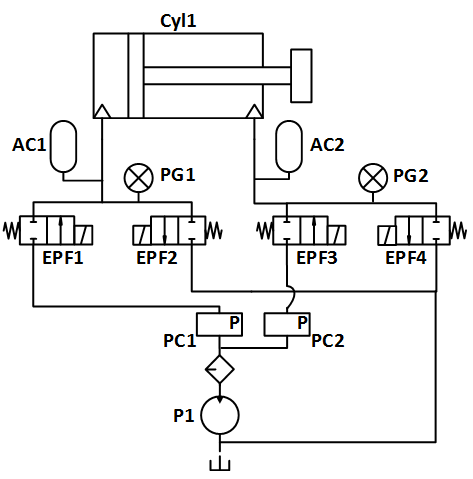
\includegraphics[width=0.45\textwidth]{imamoTAXA.PNG}
  \caption{The scheme of a hydraulic system, taken from \cite{HydroPNG}.  \label{fig:hydroSystem}}
\end{figure}
In our terminology, we could say that tags identify roles that components play in a system. Necessarily, these roles are of functional nature, for each component in an engineering system has a role in the system function. Thus, tags or, at least, the teleological content they carry, could be formalized by systemic functions. 



\subsection{Functional decomposition}\label{subsec:fun-dec}
An important feature of functions in engineering is the possibility to decompose them into sub-functions. This also allows to refine the granularity of the system description. In this paragraph, we show how such decomposition relation can be used in order to formalize the difference between \ontoFunc{fullPlural} and engineering functions that we described earlier.

First, observe that such decomposition cannot be reduced to a partial order relation between functions.  
That is, if we represent the functional decomposition of a function, say $\cst{f}$, into sub-functions, say $\cst{f}_1, \cst{f}_2, \dots, \cst{f}_n$, as $\decom(\cst{f};\cst{f}_1,\cst{f}_2,\dots,\cst{f}_n)$, then it does not seem possible to find a parthood relation such that $\decom$ reduces the mereological sum.
This is caused by, at least, the following reasons:
\begin{itemize}
  \item Functions exist at a teleological level, therefore, any decomposition of functions must take into account the decomposition of the underlying objective substrata, that is, of the underlying behaviours and objects.
  \item The sub-functions of a function must `organize'\footnote{We borrow the term from Vermaas and Garbacz \cite{vermaasFunctionalDecompositionMereology2009a}, in there the interested reader can find a discussion about mereology in functional decomposition, especially with respect to the Functional Basis methodology.} in order to realize the decomposed function. In particular, the composition of a mere set of functions is not unique.
  \item The same function can be decomposed in more ways, therefore the decomposition relation is of type many-to-many.
  \item Not all combinations of sub-functions are possible, due to physical and technical constraints. 
  Moreover, among all possible combinations, engineers recognize typical ones and use them systematically. 
\end{itemize}
Additionally, Vermaas has proven that attempting to model a Functional Basis style of functional decomposition\footnote{That is, a style where functional models can be graphically represented as directed graphs with flows as edges and function as nodes. The composition, then, can be in series, between nodes that share an edge (canceling that edge), or in parallel, between nodes that do not share edges.} entails contradictions \cite{vermaasFormalImpossibilityAnalysing2013}\footnote{The counterexamples shown are based on some additional assumptions. Precisely that, first, if a function-token is part of another function-token, then the same holds for the corresponding types; and, second, that flow loops are possible. 
}, so that there are also formal obstacles preventing the application of classical mereology to functional decompositions.
We do not attempt a solution to these problems here,
instead we assume that the relation $\decom$ is given, and focus on engineering \methodsName{plural}. 

Inspired by the work of Kitamura et al. on `ways of functional achievement' \cite{kitamuraOntologicalModelDevice2006, kitamuraOntologybasedDescriptionFunctional2003}, we consider engineering \methodsName{plural} as \methodsDefinition{plural} representing the knowledge that engineers share about ways of implementing functions through functional decomposition:
\bflist
  \item[\myax{methodSubs}] $ \Method{x} \myfi \DOLCENASO{x}$ 
\eflist
Formally, such \methodsDefinition{plural} can be understood as reifications of functional decomposition relations.
Precisely, we introduce roles $\mainFunctionRole{\cdot}$ and $\subFunctionRole{\cdot}$, contextualized by a decomposition, such that:
\bflist
  \item[\myax{main-sub-functions-sussum}] $ (\mainFunctionRole{x} \lor \subFunctionRole{x}) \myfi (\DOLCERole{x} \land \exists \cst{m} ~(\Method{\cst{m}}  \land \founded{x}{\cst{m}}))$
  \item[] \mytext{main-functions and sub-functions are roles founded on some engineering \methodsName{singular}}
\eflist 
Additionally, we assume that \methodsName{plural} are always contexts for a main-function and for a certain number of  sub-functions (axiom \refax{ax:pre-pre-method}$^*$ is actually a meta-axiom, for this reason we mark it with a $*$-symbol). 
\bflist
  \item[\myax{pre-pre-method}$^*$] $ \Method{\cst{m}} \myiff \exists! n ~\MethodBin{\cst{m}}{n},$ and $n$ is integer
  \item \mytext{Each method, say $\cst{m}$, has a (unique) number, say $n$, of  sub-functions that are contextualized by the method}
\eflist
Note that, given a finite set of methods, the previous axiom can be substituted with a finite set of axioms in FOL. The following condition constrains the decomposition relationship and is expressed via an axiom schema (here $n$ is an integer):
\bflist
  \item[\myax{pre-method}$^{schema}$] $ \MethodBin{\cst{m}}{n} \myfi \exists!  \cst{main}, \cst{sub_1}, \ldots, \cst{sub_n} (\mainFunctionRole{\cst{main}} \land \subFunctionRole{\cst{sub_1}} \land \ldots \land \subFunctionRole{{\cst{sub_n}}} \land \founded{\cst{main}}{\cst{m}} \land \founded{\cst{sub_1}}{\cst{m}} \land \ldots \land \founded{\cst{sub_n}}{\cst{m}}) $
  \item[] \mytext{for any engineering \methodsName{singular} of functional decomposition, say $\cst{m}$, having a given number of sub-functions, say $n$, there exist a main-function role and $n$ sub-function roles, which are founded on $\cst{m}$ and are uniquely determined}
\eflist
Since the main-function and the $n$ sub-functions roles of a given \methodsName{singular} are univocally determined, we can represent them with functional symbols. In particular, we will write $\cst{main^m}$, $\cst{sub}^m_1$, \dots, $\cst{sub}^m_n$ to indicate the roles corresponding to the \methodsName{singular} $\cst{m}$, as per Axiom \refax{ax:pre-method} (we omit the functional dependence of $n$ on $\cst{m}$, for ease of notation).
Finally, the link between \methodsName{plural} and decompositions is given in the following definition schema: 
\bflist
  \item[\mydf{method}$_{schema}$] $\decom(\cst{f};\cst{f}_1,\cst{f}_2,\dots,\cst{f}_n) \myiff \\ ( \FunctionSys{\cst{f}} \land \FunctionSys{\cst{f}_1} \land \ldots \land \FunctionSys{\cst{f}_n} \land \\ \exists \cst{m} (\Method{\cst{m}} \land \DOLCEConceptSubsum{\cst{f}}{\cst{main}^{\cst{m}}} \land \DOLCEConceptSubsum{\cst{f}_1}{\cst{sub}^{\cst{m}}_1} \land \ldots \land \DOLCEConceptSubsum{\cst{f_n}}{\cst{sub}^{\cst{m}}_n}) $
 \item \mytext{$\cst{f}$ is decomposed in $\cst{f_1},\ldots,\cst{f_n}$ if and only if they are all systemic functions and there is a \methodsName{singular} with corresponding main-function $\cst{main}^{\cst{m}}$ and sub-functions $\cst{sub}^{\cst{m}}_1$, \dots, $\cst{sub}^{\cst{m}}_n$, which are specialized by $\cst{f}$ and $\cst{f_1},\ldots,\cst{f_n}$, respectively}
\eflist

The advantage of this approach is manyfold: it makes possible to organize the \methodsName{singular}-types within sumbsumption taxonomies, for example, `spot welding' is a specialisation of the \methodsName{singular} `welding', which itself is an implementation \methodsName{singular} of the function `to join'; 
and to describe the properties of the \methodsName{plural}, for instance the working principle, say Kirchhoff's law for a `voltage divider' \methodsName{singular}. 
Additionally, it makes possible to introduce properties of functional decomposition. For example, if one wishes to express that all functions are decomposable, she can state:
\bflist
\item[\myex{noAtomsFunctions}] $\FunctionSys{x} \myfi \exists y~ \mainFunctionRole{y} \land \DOLCEConceptSubsum{x}{y} \land x\neq y$ 
\eflist
Instead, if one wishes to state that a function, say $\cst{f}$, is not decomposable:
\bflist
\item[\myex{yesAtomsFunctions}] $\neg \exists y~(\mainFunctionRole{y} \land \DOLCEConceptSubsum{x}{y} \land x\neq y)$
\eflist
Moreover, this approach allows us to give a formal definition of engineering function and, thereby, to discuss the ontological difference between capacities and capabilities. 
In fact, we define engineering functions to be main functions
\bflist
  \item[\mydf{engfunction}]  $ \FunctionEng{x} \myiff \mainFunctionRole{x} $
  \item[] \mytext{engineering functions and main-functions coincide}
\eflist
so that engineering functions are roles that systemic functions, which are defined in \refdf{def:function}, can play in the context of a functional decomposition.
For instance, in the lathe example discussed above, it could be that the systemic functions of the two motors are both implemented through the \methodsName{singular} of, say, `three-phase electric motor', and, therefore, play the role of engineering functions. In this case, the functional decomposition  entailed by the \methodsName{singular} includes sub-functions roles for, say, `supply electrical energy' (one per each phase), `drive the motor', and `output mechanical energy'. 


\section{Capabilities and capacities}\label{sec:CapabilAndCapac}

In this section, we discuss capabilities and capacities, two notions that we briefly introduced at the end of Section~\ref{sec:review}. In particular, we will make use of the concept of  \ontoFunc{fullSingular} to distinguish capabilities from capacities. That is, we ground the distinction on an ontological argument moving beyond views like ISO 15531-31\cite{jochemISOISO15531312004}, which proposes the association of capacities with a quantitative viewpoint and capabilities with a qualitative viewpoint only on the basis of practical arguments.

Recall that the characteristics of a technical artifact are part of its physical make-up and determine how the artifact interacts with its environment. 
For example, an individual pump is built in such a way that it is able to pump  
water with a certain flow rate.
Following the quality theory of \DOLCE, both the physical characteristics of the technical artifact and its `being able' to do something
can be conceptualized as individual qualities.\footnote{As seen in Section \ref{sec:DOLCE}, individual qualities in \DOLCE have associated quality spaces, which are essentially types of conceptual spaces as introduced in \cite{Gardenfors2004}. In the case of capabilities, which are relational qualities, the associated quality spaces should include also (at least some) dimensions relative to the entities needed for the capability to be realized.} 
Consequently, we can model the capacity `flow rate' (something that can be quantified) as a relational quality of the artifact relative to a certain kind of fluid, and the capability to pump (something that realizes a type of interaction or ability) of the same artifact as another (yet related) relational quality.
But what are these capabilities? Our theory provides a natural explanation: an entity has a capability if it can participate as doer in an \ontoFunc{fullSingular}. More precisely, an entity has a capability of a certain type (it has the capability of dividing) if and only if it can participate in the role of doer in an \ontoFunc{fullSingular} of the corresponding type (it can participate as doer in a event classified by the divide function). Thus, we assume that \ontoFunc{fullPlural} define types of capabilities, and that an entity has a capability only if it can perform (participate as doer) the corresponding \ontoFunc{fullSingular}. Starting from this level of capabilities (which we could call ontological capabilities), one can specialize capabilities to lower functional levels where functions like cutting, loading etc. are introduced, thus characterizing cutting capability, loading capability and so on.

\subsection{Capabilities vs. capacities}
Whenever a capability is based on some other quality of a technical artifact, that is, when each realisation of the capability depends on some other quality, we say that it is \firstTimeKeyWord{\foundedTerm{passive}} on that quality (or qualities). As before, we formalize this through the relation $\founded{\cdot}{\cdot}$ defined in \refdf{def:foundingBasic}.
For example, in the case of the pump we could say that the capability of the pump to move water is founded on its flow rate capacity.
Coming back to Gero and Qian's example of the water tap mentioned in Section \ref{sec:DOLCE}, which is similar to the one of the pump, we could say that the faucet has the capability of delivering water when requested, which is founded on its flow rate capacity, which is itself founded on its diameter quality (Gero and Qian say that the flow rate is \quotes{controlled} by the diameter \cite{qianFunctionBehaviorStructure1996}).
Now, in this example, there is a difference between the flow rate and the diameter: the latter is an intrinsic quality and the former is a relational quality, as we argued in Section \ref{sec:DOLCE}.
These examples suggest that  \firstTimeKeyWord{capacities} are those relational qualities on which a capability is founded, analogously to the approach in \cite{borgoCapabilitiesCapacitiesFunctionalities2021}. 
The point is that capacities are relational qualities that provide information about how the corresponding capability can be realized in practice. 
Going back to the pumping example, we conclude that the flow rate capacity  parametrizes, perhaps only partially, the pumping capability.  

Another example: electronic components such as resistors, transistors, etc., are accompanied by a datasheet that reports technical properties of the devices. 
Typical properties are, for example, the failure rate and the maximum temperature, current, or voltage that the component can reliably operate with in standard conditions. 
In our terminology, all the aforementioned properties are capacities: these properties are manifested only when the component is inserted into a working electrical circuit\footnote{As mentioned earlier in the paper, a clear-cut example is the voltage, which, since it is a potential, needs a fixed reference point in order to be measured.}; and they  parametrize some capability of the component like, say in the case of a resistor, to create a voltage drop. 

Capacities themselves are founded on some intrinsic physical qualities of the bearing object. For example, the maximum operating current will depend on the geometric and electrical properties of the conductor metal, such as its diameter and its resistivity. Similarly, the flow rate of the water tap depends on its diameter. Given these observations, we characterize capacities as follows:   
\bflist
\item[\myax{capacPartialDef}] $ \Capacity{x} \myfi \RelationalQuality{x} \land \exists y(\founded{x}{y} \land \IntrinsicQuality{y} \land \bearer{x} = \bearer{y}) $
\item[] \mytext{A capacity is a relational quality and is founded on some intrinsic quality, which is carried by the same bearer.}
\eflist
In \refax{ax:capacPartialDef}, the $\bearer{\cdot}$ is the (unique) bearer of a quality, i.e.:
\bflist
\item[\mydf{beareDef}] $ \bearer{x} = \suchthat ~\! 
y (\DOLCEQualityDirect{x}{y}) $ 
\item[] \mytext{the bearer of a quality is the entity that has (inheres) the quality}
\item[\myax{capacPartialDef2}] $ \Capacity{x} \myfi \exists y( \Capability{y} \land \founded{y}{x}) $  
\item[] \mytext{Each capacity founds a capability.}
\eflist
Axioms \refax{ax:capacPartialDef} and \refax{ax:capacPartialDef2} do not fully define what a capacity is. They only give some constraints.
Modelling the relation between capacities and capabilities remains complicated and requires further investigations. 
Yet, a promising way to tackle the problem is to define a capacity as a \quotes{parameter} of the capabilities it founds, that is, as a quality such that its values are always related to the conceptual space of the corresponding capability:
\bflist
\item[\myex{capacFullDef}] $ \Capacity{x} \myiff \RelationalQuality{x} \land \exists y,z(\founded{x}{y} \land \IntrinsicQuality{y} \land \founded{z}{x} \land \Capability{z} \land \bearer{x} = \bearer{y} = \bearer{z} \land \forall u,t (\DOLCEQualeTer{u}{z}{t} \myfi \exists v (\DOLCEQualeTer{v}{y}{t} \land \DOLCEPart{v}{u}{t}))) $ 
\item[] \mytext{Capacities are precisely those relational qualities that are founded on some intrinsic quality (of the same bearer), and which found some capability (of the same bearer), such that every time that the capability takes a range-value ($u$), the capacity takes a value ($v$) which is part of $u$.}
\eflist
Briefly put, the formula above views capacities as the parameters of capabilities allowing to ontologically support practical approaches like, e.g., that of ISO 15531-31\cite{jochemISOISO15531312004}. 

\subsection{Capabilities vs. functions}
From another perspective, capabilities are inextricably intertwined to functional aspects. 
To be able to do something is, arguably, a modal concept calling for possible events in which that something is actually done. Possible events are already part of the \DOLCE ontology so we can write the following (where $e$ is a possible, perhaps not actual, event): 
\bflist
\item[\myex{Capab}] $ \exists c(\PumpingCapability{c} \land \DOLCEQualityDirect{c}{x}) \myiff \\
\mbox{} \hfill
\exists e,t(\participateAsDoer{x}{e}{t} \land  \PumpingProcess{e}) $ 
\item \mytext{An object $x$ carries an individual capability of pumping if and only if there is a possible perdurant during which $x$ realizes some pumping process}
\eflist

Since the introduced capabilities are specifically dependent on their bearers, and each capability of a certain kind is unique to its bearer, we treat them as individual qualities.\footnote{An alternative is to model them as disposition, see for instance \cite{sarkarOntologyModelProcess2019}, and \cite{MALZKORN2001335} for a broader introduction to dispositions.} 
Finally, note that Example \refex{ex:Capab} also seems to suggest that capabilities depend on types of functions (not just processes or behaviours, for the pumping process in \refex{ex:Capab} will always play a function), which are used in their definition. This suggests to adopt the definition-founding relation already introduced in Section \ref{sec:DOLCE}: 
\bflist
\item[\mydf{capability}] $ \Capability{x} \myiff \RelationalQuality{x} \land \exists y(\FunctionAbs{y} \land \foundedDef{x}{y}) $ 
\item[] \mytext{$x$ is a capability if and only if it is a relational quality definition-founded on some \ontoFunc{fullSingular}}
\eflist
Additionally, we assume that each capability is parameterized by at least a capacity (cf. \refax{ax:capacPartialDef2}):
\bflist
  \item[\myax{capacityNuovo}] $ \Capability{x} \myfi \exists y(\Capacity{y} \land \founded{x}{y}) $
  \item[] \mytext{A capability is founded on some capacity}
\eflist
From this axiom, we have that capabilities are specifically dependent on capacities, which specify how the artifact (the bearer) can function. 
The intuition, as anticipated at the beginning of this section, is that capabilities are relational qualities that associate their bearers with \ontoFunc{fullPlural}, so that they must refer to those functions: in our terminology, they are definition-founded on \ontoFunc{fullPlural}.  
Note that they are not instantiation-founded, see \refdf{def:founding}, since an artifact could have the capability to function without actually functioning. Additionally, the function must be ontological and not systemic because, otherwise, the bearing object would be associated \textit{a priori} with some given system. 

The characterization of capacities and capabilities via \refax{ax:capacPartialDef}, \refax{ax:capacityNuovo}, and \refdf{def:capability} has the advantage of explaining:
\begin{itemize}
    \item the close link between functions and capabilities (capabilities are definition-founded on \ontoFunc{fullPlural});
    \item the asymmetry between capacities and capabilities (capabilities are founded on capacities, but not vice-versa).
\end{itemize}
The quantitative-qualitative difference between capacities and capabilities anticipated at the end of Section \ref{sec:review} is only partially clarified by this approach. For instance, while a flow-rate capability takes as values positive real numbers with, say, m$^3$/s as unit of measure, the value space of the corresponding pumping capability is quite more complex and difficult to describe. 


\medskip

One reason for the difficulty in defining capacities and capabilities is the relational and potential nature (in our interpretation) of these concepts: they are relational, and we have attempted to capture it with relational qualities, since they need the relation between their bearer and its environment to make sense; and they are potential, in the sense that they are strictly related to events that may occur, but need not to actually happen.
Functions are, arguably, similar to capabilities in this aspect, 
and this may partially explain the terminological and conceptual complexity that these concepts bring. 
Of course, these concepts are not the only ones to be both puzzling and commonly used in engineering: \textit{affordances} are another well-known example. 
As mentioned at the end of the literature review, engineering affordances are often defined as \qquotes{interaction between artifact and user in which properties of the artifact offer a potential use to the user} \cite{maierAffordanceBasedDesign2009}, but this is not an universally shared definition, and conceptual confusion persists in the disciplines (not only engineering) that make use of this concept.
We do not attempt to carry out an ontological analysis of affordances, but we do make two brief observations:
\begin{itemize}
  \item first, the reasons for the confusion around the concept of affordance may be, at least partially, the same for the concepts analyzed in this paper. They strongly depend on relations between entities, and they are potential concepts, as opposed to actual.
  \item Second, one could attempt to reduce affordances to capabilities using, for example, the following informal equivalence:
  \bflist
    \item[\myex{affordances}] \mytext{An engineering artifact affords a user (or another artifact) to do something if and only if the system made by the artifact, the user (or the second artifact), and their relation has the capability to do that something}
  \eflist 
\end{itemize}
From this point of view, our analysis of capabilities would carry at least some insight into affordances.

Finally, in Figure \ref{fig:model} we give a schema that shows the main relations and concepts used in our theory of engineering functions.

\begin{figure}
    \centering
    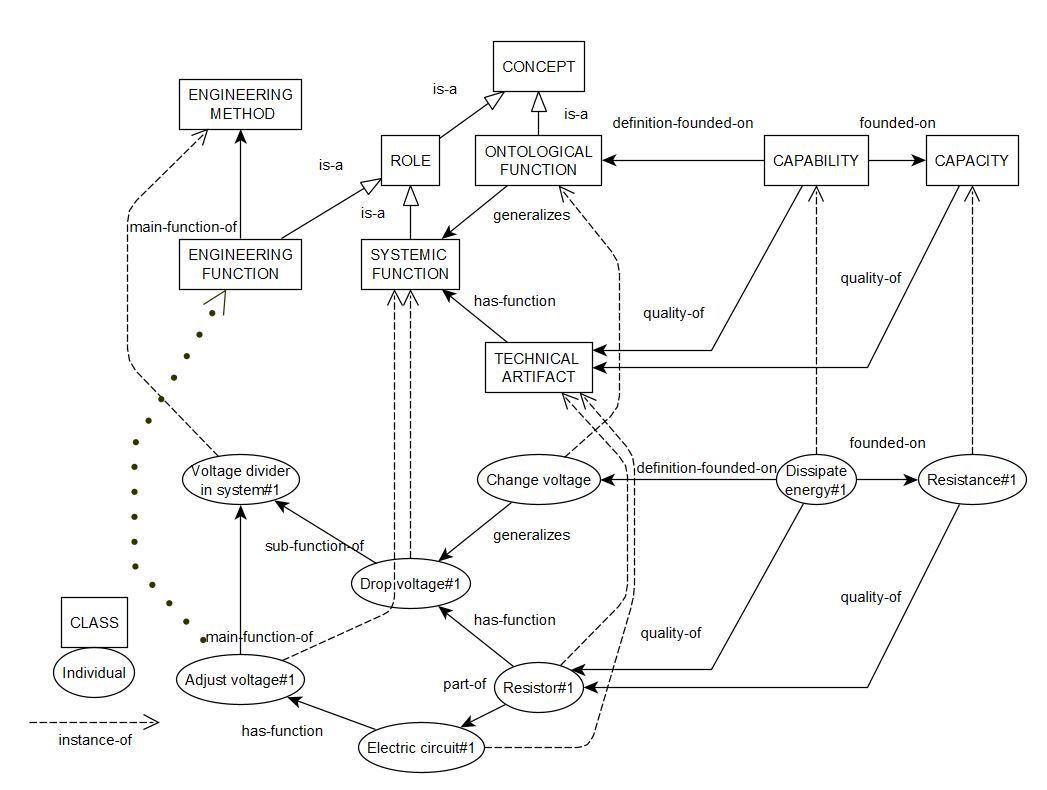
\includegraphics[width=0.95\textwidth]{schema-manual-nocolorv2.JPG}
    \caption{Main concepts and relations in the presented ontology. For simplicity and clarity, the picture refers to the OWL model and many relations and concepts have been suppressed. In addition, an instantiation of the schema for the case of a voltage divider is given. The dotted instance-of arrow is inferrable, since the related systemic function is main-function-of some engineering method (cfr. \refdf{def:engFunc}).}
    \label{fig:model}
\end{figure}

\medskip
We conclude this section with another example to show how the concepts we have introduced above concur to provide an integrated description of a functional scenario. Suppose that a company handling swimming pools must empty some of its pools for maintenance. This imposes a goal, say `the pools are empty', that must be carried out through some device able to realize a `to move' (ontological) function, specialized to a systemic function in the context of the swimming pool system.
Such a function can be realized by artifacts that have a corresponding capability. In this case, the function would probably be implemented through some fluid-emptying-method, that is, through the knowledge of the way that a recipient can be emptied, and its fluid content disposed of, by pressurizing the fluid and guiding it through a path.
Now, the `pressurize' sub-function (which refers to the goal of `having a big enough pressure gradient') could be implemented through a pumping-method, that is, referring to engineering knowledge about pumps.
Then, a pump (more generally an artifact with pumping capability) could be selected for being the `doer' of the necessary `transform electrical energy into pressure' sub-sub-function.
In this context, we could say that the pump has been selected because of its pumping-capability and that the pumping-method describes, at least, a flow rate capacity, which founds the pumping-capability, and its interaction to the other properties and entities involved in the pumping process. 



\section{Evaluation and possible applications}\label{sec:appendice}
\subsection[meta]{Reduction to \OWL ontology}
To facilitate the deployment of our theory in applications, we present an \OWL version of the first-order logic formalization. 
This is standard practice, for at least the following reasons: first, \OWL is decidable, while first-order logic is not, so that reasoning tasks will terminate in finite time.\footnote{Though the complexity might be  exponential in general.} Second, \OWL is a standard endorsed by the World Wide Web Consortium (W3C) and is part of the Semantic Web technology stack \cite{OWL2-QUICK-REFERENCE}, and is the language of choice for many ontologies in various domains \cite{OWL-ontology-repositories}.

Unfortunately, the computational properties of \OWL come with a tradeoff with respect to its expressibility, therefore, one has to simplify the first-order theory. 
The original theory remains essential as it constrains the intended meanings of the \OWL concepts and provides the `official reading' of the theory, it also helps to conceptually understand how the overall model is supposed to work. 

The first-order theory developed in the previous sections can be converted to \OWL language as is, except for the expressions where ternary relations are used, as well as those that necessarily need at least three arguments to be formulated. 
For example, the definition of systemic-function-of \refdf{def:functionOf}, the instantiation-founding definition \refdf{def:founding}, and the engineering \methodsName{singular} schema \refdf{def:method} cannot be expressed in \OWL. 
In these cases we have to weaken the axioms. For instance, in \OWL we replace the definition of systemic functions with
\bflist
\item[\myax{functionOWL}$_{owl}$] 
\myalignspaceskip
\setlength{\jot}{0pt}
\begin{align*}
    \FunctionSysNullary\sqsubseteq &
    (\forall\mathtt{classifies}.\BehaviourConcreteNullary \sqcap \exists\causallyContrNullary.\GoalNullary) 
        \sqcap \\ & \exists\foundedNullary.\SystemNullary)
\end{align*}
\eflist
where $\mathtt{classifies}$ is the inverse relation of $\DOLCECLby{\cdot}{\cdot}{\cdot}$. In this way the fact that systemic functions are founded on systems is preserved. 

Additionally, all the ternary temporalized relations used in the first-order version, such as $\DOLCECLby{\cdot}{\cdot}{\cdot}$ 
and $\hspace{0pt}\texttt{participateAsDoer}(\cdot,\cdot,\cdot)$, occur in the \OWL version with the temporal argument removed, i.e., as binary relations.
The link between the temporalized and non-temporalized relations can be interpreted in different ways \cite{TerkajOntologyIndustrialEngineering2022}. For example, one could state that the non-temporalized relation holds if and only if the temporalized relation holds whenever one of the relation arguments exists, what argument precisely depends on the relation. This is our choice for parthood \refdf{def:partConstant}, classification, temporal quale, and participation-like relations as shown by these \textit{meta-rules} aimed to show the intended interpretations: 
\bflist
\item[\mydf{CLnontemp}$_{meta}$] $ \DOLCECLbyBinary{x}{y} \myiff ((\exists t \DOLCEPRE{x}{t}) \land \forall t (\DOLCEPRE{x}{t} \myfi  \DOLCECLby{x}{y}{t}))$ 
\item \mytext{$x$ is constantly classified by $y$ if and only if $x$ is classified by $y$ whenever $x$ exists}
\item[\mydf{Qualenontemp}$_{meta}$] $ \DOLCEQualeDirect{x}{y} \myiff ((\exists t \DOLCEPRE{x}{t}) \land \forall t (\DOLCEPRE{x}{t} \myfi  \DOLCEQualeTer{x}{y}{t}))$ 
\item \mytext{$y$ is a constant temporary quale of the quality $x$ if and only if $y$ is a temporary quale of $y$ whenever $x$ exists}
\item[\mydf{participationDoerNonTemp}$_{meta}$] $ \participateAsDoerBinary{x}{y} \myiff \exists t (\DOLCEPRE{y}{t}) \land \forall t (\DOLCEPRE{y}{t} \myfi \participateAsDoer{x}{y}{t})$
\item \mytext{$x$ constantly participates-as-doer to $y$ if and only if $x$ participates-as-doer to $y$ for the whole of $y$ duration}
\eflist
One could also state that the non-temporalized relation holds if and only if the temporalized relation holds true at some time adopting the following \textit{meta-rule}: 
\bflist
\item[\myex{participationDoerNonTempBIS}$_{meta}$] $ \participateAsDoerBinary{x}{y} \myiff \exists t ~\participateAsDoer{x}{y}{t}$
\eflist
There are other possibilities. The choice of one over the others must be planned carefully depending on the application concerns, since this kind of changes affects the intended models of the \OWL ontology. For example, \refdf{def:participationDoerNonTemp} excludes participation-as-doer in, say, a chemical process only for its first part, while \refex{ex:participationDoerNonTempBIS} allows it, but in \OWL this difference is lost.
Additionally, the removal of the temporal argument reduces the flexibility of the ensuing ontology. For example, one cannot track (at least not directly) dynamic aspects of roles, e.g. a component that carries out a function at a time and then it changes its function. Nor one can express that, say, there is a chemical process which is driven by two different catalysts during its first and second parts.

Finally, as a further simplifying assumption, we define two binary relations that we will use as shortcuts to implement and simplify the definition schema  \refdf{def:method} and to redefine \refdf{def:engfunction}:
\bflist
  \item[\mydf{main-function-of}$_{meta}$] $ \mainFunction{\cst{f}}{\cst{m}} \myiff (\DOLCEConceptSubsum{\cst{f}}{\cst{main}^{\cst{m}}} \land \FunctionSys{\cst{f}}) $
  \item \mytext{$\cst{f}$ is main-function-of a \methodsName{singular} $\cst{m}$ if and only if it is a systemic function specializing the main-function role correspondig to $\cst{m}$} 
  \item[\mydf{sub-function-of}$_{meta}$] $ \subFunction{\cst{f}}{\cst{m}} \myiff (\DOLCEConceptSubsum{\cst{f}}{\cst{sub}^{\cst{m}}_i} \land \FunctionSys{\cst{f}}) $
  \item \mytext{$\cst{f}$ is main-function-of a \methodsName{singular} $\cst{m}$ if and only if it is a systemic function specializing any of the sub-function roles correspondig to $\cst{m}$} 
  \item[\mydf{engFunc}$_{owl}$] $ \FunctionEngNullary\equiv \exists\mainFunctionNullary.\MethodNullary$
  \item \mytext{Engineering functions are exactly the individuals that are main-function-of some engineering method}
\eflist

Note that in \refdf{def:engFunc} the individuals must necessarily be systemic functions due to \refdf{def:main-function-of}.

\begin{figure}[t]
  \centering
  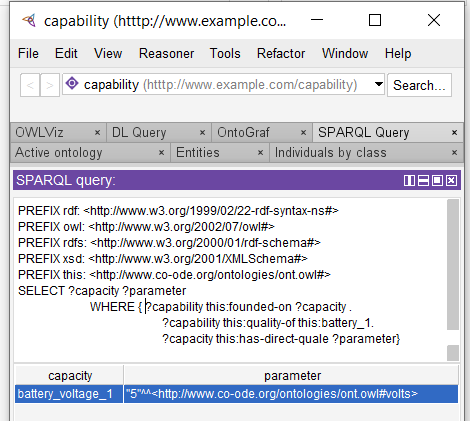
\includegraphics[width=0.7\textwidth]{query_screenshot.PNG}
  \caption{An implementation of \refCQ{CQ:capability-founded} in Protegé.\label{fig:screen_query}}
\end{figure}

\begin{figure}
  \centering
  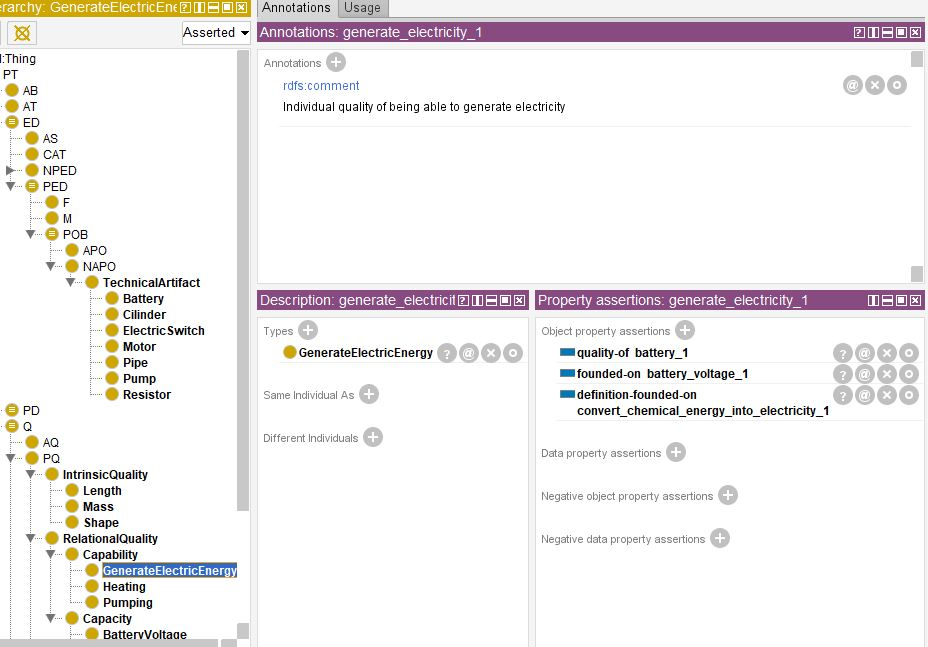
\includegraphics[width=0.8\textwidth]{entities_screenshotv2.JPG}
  \caption{A view of the ontology taxonomy in Protegé.\label{fig:screen_entities}}
\end{figure}

Even though the \DOLCE ontology is primarily a first-order logic theory, \OWL versions exist as well, e.g. \DOLCE-lite and \DOLCE-Ultralite.\footnote{Available at \url{http://www.loa.istc.cnr.it/index.php/dolce/}.}
Any of these could be used to align the ontology developed in this paper with \DOLCE. In our case, we used the \OWL version of \DOLCE that has been recently submitted as part the ISO 21838 standard. 
The resulting ontology, which can be found on GitHub\footnote{\url{https://github.com/kataph/function-method-ontology.git}.}, was tested using the Hermit reasoner.
(For the sake of example, the ontology is populated with only a few individuals).


\subsection{Evaluation}
The ontology developed in this paper is a hand-crafted prototype that discusses middle and high-level concepts. 
Therefore, some common approaches to evaluation cannot be employed, as, for example, there is no \qquotes{gold standard} \cite{sfarGoldStandardBased2016}, or set of formal ontologies that one could use to compare common ontology metrics (such as those extracted by OntoMetrics\footnote{\url{https://ontometrics.informatik.uni-rostock.de/ontologymetrics/index.jsp}.}), nor there is a precise application against which to carry out the evaluation. 
Instead, we will evaluate our ontology using the OntoClean methodology  \cite{guarinoOverviewOntoClean2009} and the Ontology Pitfall Scanner \cite{poveda2014oops}. 
Moreover, we will discuss how our ontology answers the research questions \refRQ{RQ:RQ1}-\refRQ{RQ:RQ1.2}, as well as some competency questions that will serve to demonstrate the expressive potential of the ontology.
Finally, we will also discuss some possible application scenarios, though we highlight that the ontology main goals are the research questions \refRQ{RQ:RQ1}-\refRQ{RQ:RQ1.2}. The development of derived application-level ontologies is a goal for further work.

\paragraph{OntoClean.} OntoClean does not identify any issue in our taxonomy, that is, none of the meta-level rules that OntoClean methodology enforces are violated.
In fact, this is almost trivial to check: since we are extending \DOLCE categories, the only source of OntoClean violations would be an extension of role-concepts (that is, the set of all entities that, at a given time, are classified by the role-concept) which is not anti-rigid. 
This condition is not violated since (systemic) functions, as we define them, are contextual (e.g., a heat exchanger, with its behaviour, may be used either to heat a substance or to cool it, depending on the context). The other rules checked in the OntoClean methodology are trivially true. 
The correspondence with OntoClean principles is mainly due to the alignment of our theory with a well-established upper-level ontology. 

\paragraph{Ontology Pitfall Scanner} The \OWL ontology was evaluated with the Ontology Pitfall Scanner (OOPS!) \cite{poveda2014oops}, which searches for common design errors from a list of 41 items. Among the pitfalls not related to imported ontologies, the scanner found some minor stylistic issues\footnote{Some inverse object-properties are not declared explicitly, and the naming convention differs between object-properties and classes.} and warned about a few important pitfalls: P11 (\qquotes{Missing domain or range in properties}), P24 (\qquotes{Using recursive definitions}), and P30 (\qquotes{Equivalent classes not explicitly declared}). Of these three, P11 means that not every object property has domain and range axioms, but this is a conscious design choice to reduce the ontological commitment of the ontology. P24 occurs because OOPS! thinks that \refax{ax:functionAbstr} is a recursive definition (since the class of ontological functions appears both on the left and on the right of the material implication), but this is not the case. 
Similarly, P30 occurs because OOPS! is, incorrectly, assuming that the class of resistors (capabilities) and the class of resistances (capacities) should be equivalent. 

\paragraph{Research questions and competency questions}
Our ontology answers the research questions listed in the introduction. 
In particular:
\begin{itemize}
  \item \textbf{Answer to \refRQ{RQ:RQ1}.} We modeled functions as \DOLCE-concepts that classify certain classes of perdurants. 
  This modelling choice explains how functions can exist even when they are not executed.
  Moreover, we separated functions into the distinct categories of engineering methods and (proper) functions, and, further, we separated functions into systemic or ontological depending on their abstraction level, thus explaining the ambiguity on the why-how or abstraction-implementation axes.
  \item \textbf{Answer to \refRQ{RQ:RQ1.1}.} Systemic functions can be decomposed as discussed in Subsection \ref{subsec:fun-dec}, where each decomposition is associated with an engineering \methodsName{singular}. 
  \item \textbf{Answer to \refRQ{RQ:RQ1.2}.} We have characterized capabilities and capacities in Section \ref{sec:CapabilAndCapac}. In the first case we leveraged ontological functions, in the second case we suggested considering capacities as parameters of capabilities. Moreover, capabilities and capacities are clearly separated by the use of the founding relation: capabilities are founded on capacities, while the opposite does not hold.     
\end{itemize} 
Additionally, since the formal ontology answers these research questions, it is also able to answer related competency questions, which can be of interest in applications, such as the following:

\bflist
\item[\myCQ{first-function-capability}] Given an (ontological) function, which artifacts have the capability of satisfying it? 
\item[\myCQ{function-implementation}] How can the given ontological function be implemented? 
\item[\myCQ{capability-founded}] What are the capacities that a given capability is founded on?
\item[\myCQ{function-parameter2}] Which parameters explain the performance of the some component in a given system? (If interpreted as \quotes{what are the capacities of the capabilities of the component that are relevant in executing its function?})
\item[\myCQ{function-decomposition}] Which is the functional decomposition of a given system? 
\item[\myCQ{last-tag-function}] Which is the function of the given tag and what is its purpose?
\eflist


The \OWL ontology, after being populated, can be used to answer the competency questions \refCQ{CQ:first-function-capability}-\refCQ{CQ:last-tag-function} by means of SPARQL queries. 
For example, these are implementations of \refCQ{CQ:first-function-capability}:
\begin{verbatim}
  PREFIX : <https://github.com/kataph/function-method-ontology#>
  SELECT  ?component
  WHERE { 
    ?capability :definition-founded-on :<the given function> .
    ?capability :quality-of ?component}
\end{verbatim}
of \refCQ{CQ:function-parameter2}:
\begin{verbatim}
  PREFIX : <https://github.com/kataph/function-method-ontology#>
  SELECT  ?component ?functionOntological ?capacity
  WHERE { 
          ?functionSystemic :function-of ?component .
          ?functionSystemic :founded-on :<the given system> .
          ?functionSystemic :specializes ?functionOntological .
          ?capability :definition-founded-on ?functionOntological .
          ?capability :quality-of ?component .
          ?capability :founded-on ?capacity .
          ?capacity :quality-of ?component}
\end{verbatim}
and of \refCQ{CQ:function-decomposition}, provided that the functional decomposition of a system is interpreted as the list of all systemic functions of the given system involved in a \methodsName{singular}, with their role (main-function or sub-function) and underlying component:
\begin{verbatim}
  PREFIX rdf: <http://www.w3.org/1999/02/22-rdf-syntax-ns#>
  PREFIX rdfs: <http://www.w3.org/2000/01/rdf-schema#>
  PREFIX : <https://github.com/kataph/function-method-ontology#>
  SELECT  ?component ?functionSystemic ?role ?method 
  WHERE { 
      ?functionSystemic ?role ?method .
      ?method rdf:type/rdfs:subClassOf* :EngineeringMethod .
      ?functionSystemic :function-of ?component  .
      ?component :constant-part-of :<the given system>}
\end{verbatim}
The remaining competency questions can be implemented in a similar way (see also Fig.\ref{fig:screen_query} for \refCQ{CQ:capability-founded}).

\medskip
The fact that our ontology can answer all these questions shows its expressivity and coverage.
In the following paragraphs we explain how these characteristics could be used in application scenarios.


\subsection{Motivating scenarios}
\paragraph{Innovative Design (and other things).}
A good portion of the literature on functional modelling argues that functional modelling can be used to improve engineering design.
For instance, the basic argument of the approach of Pahl and \cite{pahl_engineering_2007} is as follows: designers should start from the customer's requirements, translate them into high-level functions, then decompose those functions into less abstract ones, until arriving at a point where finding a solution that realizes the functions is easy.
This methodology, is argued, facilitates engineers to quickly develop high-quality designs and enhances their creativity by decoupling the goals of the design from the ways they are achieved.

This argument is not wrong, but, in actual practice, one rarely starts from a blank slate. 
Designers are typically constrained by the need to reuse pre-existing solutions, for a company may have developed a legacy that is difficult to depart from, possibly because the company would not be able to (profitably) reroute its know-how and resources towards innovative lines of products, or other reasons.
Therefore, designers usually have to devise marginal improvements or corrections in pre-existing solutions, and these activities seem at odds with the aforementioned methodology. 
Additionally, the described methodology is design-oriented and does not seem relevant to other activities, such as troubleshooting or reverse engineering, despite functional reasoning being clearly relevant in all of them.

One important reason for carrying out ontological analysis is to bridge all such activities and cases, by producing an explicit representation (the ontology) of the shared conceptualisation of the relevant stakeholders, which can be used by all of them.
We argue that our ontology is useful for the blank-slate innovation scenario (for, e.g., competency questions \refCQ{CQ:first-function-capability} and \refCQ{CQ:capability-founded} showcase the possibility of linking capabilities to functions, which is important since it allows engineers to find whether they already have available components that can satisfy a given functional requirement), as well as many other scenarios, some of which we describe briefly in the following. 

\paragraph{Incremental innovation} In a company, innovation may happen mainly through incremental changes in pre-existing products. 
Therefore, product types will have a version history. 
Using our ontology, one could describe 
the relevant improvements, allowing their digitalisation in a semantically meaningful way. 
For instance, a new version may introduce new capabilities, or it may have the same capabilities as the former version, but it could realize them better due to different capacities. 
Storing such information could be more helpful to engineers than just storing structural information (like the bill of material) of the different versions in the enterprise management system.

\paragraph{Knowledge transfer} An engineer or technician could have recently been employed by a manufacturing company. 
In that case, he or she is (hopefully) trained to learn about the company's products and their functioning. 
Still, a good part of the knowledge the company possesses, especially functional knowledge, is implicit. 
Therefore, the trainee will learn about it only through experience or through his/her background knowledge of the domain. 
This may be a slow process, and some knowledge could be lost. 
Building a knowledge base modelling functional knowledge (necessarily together with other types of information, e.g. geometrical from CAD models, etc.) could facilitate training since it would relieve the trainee from having to infer the functionality of components from their structure, as well as the (functional) role of components within their systems. 

\paragraph{Troubleshooting} When a technician troubleshoots a product he often makes use of functional reasoning (e.g., \qquotes{the volume of the speakers is constantly louder than it should be. It may be that there is something wrong with the amplifier circuit, since it is that component that has the function of controlling the volume}). 
Sometimes, a technician may lack sufficient knowledge about the functional structure of a product to carry out such reasoning fruitfully (say, it is an external contractor with limited knowledge of the company which manufactures the product). 
In those cases, a clear rapresentation of the product functional structure, if accessible to the technician, may solve the issue.
For example, a query answering \refCQ{CQ:function-parameter2} may be useful in this  case.

\paragraph{Formal Requirements.}
Requirements are an essential part of engineering design, which engineers have to write, share, maintain, and implement. 
The ensuing work and documentation can be daunting, especially in large progects. Therefore, attempts have been made to standardize \cite{alrumaihDomainOntologyRequirements2020}, trace \cite{murtazinaOntologybasedApproachSupport2019}, and automatize \cite{holterScopeDetectionTextual2021} requirement pipelines using ontologies. 
Some approaches discuss how requirements should be written, so that their quality, shareability, and even automatic verification against a design model can be assured (e.g., \cite{jinxinlinRequirementOntologyEngineering1996, chenOntologybasedRequirementVerification2020}).
In the latter case, requirements are usually interpreted as assertions (constraints) about an engineering artifact that can be expressed (at least some of them can) in a formal language. 
The fact that the requirement refers to something that \textit{should be}, and not to something that \textit{is}, means that requirements are modal concepts, though this can be left implicit in formal representations.  
For example, a requirement translated directly from a client's request, could be that the product, say a table, \qquotes{must weight as little as possible}, then engineers could precise this in different ways, e.g., by stating 
\bflist
  \item[\myex{req1}] $ weight(table\_top) \leq 5kg \land weight(i_{th}\_table\_leg) \leq 2kg$, for $i = 1,2,3,4$. 
\eflist
Therefore, if one also designs products using the same formal language, the products can be checked against the set of constraints, to verify that those are satisfied by the products.

One difficulty of this approach is that some requirements are more difficult to express than others.
Requirements such as \refex{ex:req1} are easy to express, as they refer to physical properties of the products (they are sometimes called \qquotes{physical requirements} \cite{jinxinlinRequirementOntologyEngineering1996}).
On the other hand, requirements linked to product performance or functions are more difficult to express.
For example, in \cite{jinxinlinRequirementOntologyEngineering1996}, the requirements \qquotes{The artifact [desk spot lamp] should be able to illuminate more than half a square meter of room}, \qquotes{The base [of the desk spot lamp] should provide support to the artifact}, and \qquotes{the short arm must have a hole [\dots]} are formalized as follows: 
\bflist
  \item[\myex{req2}] $ arm(p) \myfi \exists f(hole\_feature(f) \land
 feature\_of(f, p) \land
  $ [\dots]. 
  \item[\myex{req3}] $ desk\_spot\_lamp(p) \myfi \exists f( illuminating\_feature(f) \land feature\_of(f, p) \land illumination\_area(f) \geq 0.5 $
  \item[\myex{req4}] $ base(p) \myfi \exists f (provide\_support\_feature(f) \land feature\_of(f, p) $ 
\eflist
Therefore, predicates \qquotes{$illuminating\_feature$}, \qquotes{$provide\_support\_feature$}, and \qquotes{$hole\_feature$} are introduced to classify the capability to illuminate, the function to support, and the hole of the short arm as \qquotes{$feature\_of$} the corresponding artefacts. 
So that capabilities and functions are features in the same sense that a hole is, and we consider this an ontological error\footnote{For example, in \DOLCE features form a category of endurants that are (generically constantly) dependent on physical objects that cannot be detached from their corresponding physical object without losing their identities. In this sense, a hole is a feature, while the wheel of a car is not. The fact that, in our approach, features are not capabilities or functions, entailed by our categorisation of those as qualities and non-physical endurants, respectively.}.

The point is that being able to express requirements that mention capabilities or functions is difficult, and an ontology describing such concepts would make things easier.
For example, using our theory we would write requirements \refex{ex:req3} and \refex{ex:req4} as, respectively (in the following we have introduced a subclass of capabilities, $illuminating\_capability$, a subclass of capacities $illumination\_area$, and a subclass of (ontological) functions, $provide\_support$):
\bflist
  \item[\myex{req5}] $ desk\_spot\_lamp(p) \myfi \exists f,c,v( illuminating\_capability(f) \land \DOLCEQualityDirect{f}{p} \land illumination\_area(c) \land \\ \founded{f}{c} \land \DOLCEQualeDirect{c}{v} \land \DOLCEPartBin{v}{[0.5, \infty)}$
  \item[] \mytext{Every desk spot lamp has a capability to illuminate, founded on an illumination-area-capacity greater than 0.5} 
  \item[\myex{req6}] $ base(p) \myfi \exists f_o,f_s (provide\_support(f_o) \land \DOLCECLbyBinary{f_s}{f_o} \land \FunctionSysOf{f_s}{p})$
  \item[] \mytext{Every lamp base has a (systemic) function of (ontological-function-)type provide support} 
\eflist
Notice that \refex{ex:req5} and \refex{ex:req6} can be readily rewritten in \OWL, so that they can be part of an \OWL knowledge base containing all the requirements that can be expressed in a similar way. 
Then, if engineers build during design a model of the product, using the same language, they just need to import the model into the knowledge base with the requirements: the product model satisfies the requirements if and only if the ensuing ontology is consistent (similarly one can find if the requirements are inconsistent or if there are duplicates).  
In an actual application the user may never write complex formulas such as \refex{ex:req5} and \refex{ex:req6}, unless user-friendly templates are made available as done in \cite{chenOntologybasedRequirementVerification2020}.  

An analogous procedure is the one that the READI project \cite{overliAssetInformationModelling2021,kluwerOntologybasedRequirementsManagement2018} aims to implement. 
In their case, the requirement are expressed in SCD (Scope Condition Demand) form.
This means that they are assertions of the form
\bflist
  \item[\myex{SCD}] $ \text{S} \sqcap \text{C} \sqsubseteq \text{D}  $
\eflist
where S, C, and D are \OWL classes, for example (the example is taken from \cite{overliAssetInformationModelling2021}), \qquotes{Equipment with a transport dry weight above 1000 kg shall be weighed by the manufacturer and a weight certificate shall be issued} is written in such a form, if S, C, and D are interpreted as the classes \quotes{Equipment}, \quotes{things with transport dry weight above 1000 kg}, \quotes{things that have a weight certificate}, respectively.   
Again, it is difficult to express functions- and performance-related requirements in the format of \refex{ex:SCD} if one lacks an appropriate reference ontology. 


\section{Conclusion}\label{sec:conc}
The work presented in this paper contributes to the ontological understanding and modeling of fundamental concepts used in engineering, especially functionality.
In particular, we have shown how one can give ontologically-grounded definitions of capability, capacity, behaviour, and function using first-order logic.
Moreover, we have shown how one can use an ontology and the notion of functional decomposition to distinguish between ontological, systemic, and engineering functions, and how \ontoFunc{fullPlural} can be used to explain the difference between capabilities and capacities.
Finally, we partially translated our first-order theory in \OWL, showcasing a preliminary serialisation of our theory in a computer-friendly formal language.

Our approach builds on a series of previous works, especially on the study of functionality carried out by engineers and researchers, in particular \cite{pahl_engineering_2007, sasajimaFBRLFunctionBehavior1995,mizoguchiUnifyingDefinitionArtifact2016}; the study of resources in manufacturing, in the applied ontology literature as well as some standards  \cite{sanfilippoResourcesManufacturing2015, borgoCapabilitiesCapacitiesFunctionalities2021, jochemISOISO15531312004}; and the top-level ontology \DOLCE and its developments \cite{masoloSocialRolesTheir2004, masoloWonderWebDeliverableD182003,borgoDOLCEDescriptiveOntology2022}.
This work relies on an in-depth ontological analysis of the domain, which,  exploiting the characteristics of the \DOLCE ontology, clarifies the conceptualisation of functions and related concepts in a systematic way.

We evaluated the quality of our implementation by assessing the clarity, expressive capability, and flexibility of our ontology with respect to some research questions, some competency questions, and some application scenarios. 
The relevance of our work is highlighted by the ability to answer a series of questions, from \refRQ{RQ:RQ1}-\refRQ{RQ:RQ1.2} to \refCQ{CQ:first-function-capability}-\refCQ{CQ:last-tag-function}, showing that the ontology could be able to support applications in most engineering scenarios where functional reasoning is required. 

This paper has set the vision and the core elements of our theory, yet many things require further work and testing to achieve a  level of detail and coverage suitable for real applications.
For example, linking the notions of behaviour to the modelling equations that engineers use to simulate a system is a topic that has not been addressed and requires additional research. Similarly, we need to analyze more in-depth how an ontological approach based on our theory can help to make uniform the description of application scenarios, starting from those touched upon in the paper.





\section*{Acknowledgments}


The authors acknowledge support by the European project OntoCommons (GA 958371, \url{www.ontocommons.eu}). Francesco Compagno is funded by the company Adige Spa. 
The authors wish to thank Riichiro Mizoguchi for the precious time spent discussing his work as well as the topics of function definition and engineering function modelling.





\bibliographystyle{ios1}           
\bibliography{bibliography}        

\end{document}
